\documentclass[twoside]{book}

%---------------------------------------------------------------
%   PACKAGES
%---------------------------------------------------------------
\usepackage{graphicx} % Required for inserting images
\usepackage{xcolor}
\usepackage{acronym}
\usepackage{tabularx}
\usepackage{longtable}
\usepackage{colortbl}
\usepackage{float}
\usepackage{listings}
\usepackage{rotating}
\usepackage{hyperref}

%---------------------------------------------------------------
%   ALLOY CONFIG
%---------------------------------------------------------------
\lstdefinelanguage{alloy}{
    morekeywords={
        module, open, as,
        private, abstract, sig, extends, in,
        lone, some, one, disj,
        fact, pred, fun, assert,
        run, check,
        for, but, exactly,
        this, not, implies, else, let,
        not, no, set, all, sum,
        iff, or, Int, and,
        none, univ, iden
    },
    sensitive=true,
    morecomment=[l]{//},
    morecomment=[l]{--},
    morecomment=[s]{/*}{*/},
    morestring=[b]{"},
%literate={->}{$\rightarrow$}1
% replacing characters can cause problems when copying from PDF to editor
}[keywords,comments,strings]

\definecolor{dkgreen}{rgb}{0,0.6,0}
\definecolor{gray}{rgb}{0.5,0.5,0.5}
\definecolor{mauve}{rgb}{0.58,0,0.82}


\lstset{frame=tb,
    language=alloy,
    aboveskip=3mm,
    belowskip=3mm,
    showstringspaces=false,
    columns=flexible,
    basicstyle={\small\ttfamily},
    numbers=none,
    numberstyle=\tiny\color{gray},
    keywordstyle=\bf\color{blue},
    commentstyle=\it\color{dkgreen},
    stringstyle=\color{mauve},
    breaklines=true,
    breakatwhitespace=true,
    tabsize=3
}

%---------------------------------------------------------------
%   NEW COMMANDS
%---------------------------------------------------------------

\newcommand{\newtext}[1]{\textcolor{blue}{#1}}
\newcommand{\myworries}[1]{\textcolor{red}{#1}}

%---------------------------------------------------------------
%   ACRONYMS
%---------------------------------------------------------------


\acrodef{CKB}[CKB]{CodeKataBattle}
\acrodef{CK}[CK]{CodeKata}
\acrodef{UI}[UI]{User Interface}
\acrodef{SOA}[SOA]{Service Oriented Architecture}
\acrodef{API}[API]{Application Programming Interface}
\acrodef{HTML}[HTML]{}
\acrodef{CSS}[CSS]{}
\acrodef{JS}[JS]{JavaScript}
\acrodef{DBMS}[DBMS]{DataBase Management System}
%---------------------------------------------------------------
%   DOCUMENT
%---------------------------------------------------------------

\begin{document}


\title{DD}
\author{Federico Valentino, Nicola Zarbo }
\date{October 2023}


\maketitle
\newpage
\setcounter{page}{1}

\tableofcontents % Table of contents
\cleardoublepage

\chapter{Introduction}
\section{Purpose}
\ac{CKB} is a new platform that helps students improve their software development skills by training with peers on code katas . Educators use the platform to challenge students by creating code kata battles in which teams of students can compete against each other, thus proving (and improving) their skills.\newline
A code kata battle is essentially a programming exercise in a programming language of choice (e.g., Java, Python). The exercise includes a brief textual description and a software project with build automation scripts (e.g., a Gradle project in case of Java sources) that contains a set of test cases that the program must pass, but without the program implementation. Students are asked to complete the project with their code. In particular, groups of students participating in a battle are expected to follow a test-first approach and develop a solution that passes the required tests. Groups deliver their solution to the platform (by the end of the battle). At the end of the battle, the platform assigns scores to groups to create a competition rank.
\subsection{Goals}
The \ac{CKB} system is thought, designed and proposed to two types of users: Students and Educators.\newline
The firsts, will be able to join the platform to test their coding skills in Tournaments, a series of code battles, where students will be able to participate in groups.\newline
Educators instead will be able to create and manage tournaments and decide whether or not a manual score in a battle is needed or not.\newline
Below the list of goals of the \ac{CKB} platform.\newline

\begin{center}
    \begin{longtable}{ |l|p{0.9\linewidth}| }
        \hline
        \textbf{ID} & \textbf{Description}\\
        \hline
        G1 & An Educator can manage a tournament. \\
        \hline
        G2 & An educator can create battles inside of a tournament in which he is involved. \\
        \hline
        G3 & Students can participate in tournaments created by an educator\\
        \hline
        G4 & Students can participate and compete in battles created by an educator, alone or in groups. \\
        \hline
        G5 & Students are scored based on their performance in battles. \\
        \hline
        G6 & The platform allows students and educators to compare the performance of students. \\
        \hline
        \caption{The goals.}
    \end{longtable}
\end{center}


\section{Scope}
\subsection{World phenomena}
\begin{center}
    \begin{longtable}{ |l|p{0.9\linewidth}| }
        \hline
        \textbf{ID} & \textbf{Description}\\
        \hline
        W1 & An educator wants to create a tournament to evaluate students performance. \\
        \hline
        W2 & Students fork the created repository for a battle on Github. \\
        \hline
        W3 & An educator creates the battle assignment. \\
        \hline
        W4 & Students write source code for the code kata battle. \\
        \hline
        W5 & Students create commits on Github. \\
        \hline
        W6 & Students decide to join a battle. \\
        \hline
        W7 & Students create groups for battles. \\
        \hline
        W8 & Students setup an automated workflow for the forked repository on Github. \\
        \hline
        W9 & Students decide to join a tournament. \\
        \hline
        W10 & Educator decides to close tournament. \\
        \hline
        \caption{World Phenomenas.}
    \end{longtable}
\end{center}
\subsection{Shared phenomena}

\begin{center}
    \begin{longtable}{ |l|p{0.5\linewidth}|l|l| }
        \hline
        \textbf{ID} & \textbf{Description} & \textbf{Controller} & \textbf{Observer}\\
        \hline
        SP1 & An educator fills out a tournament creation form. & Educator & \ac{CKB}\\
        \hline
        SP2 & An educator uploads the details of a code kata battle(the assignment, the rules, the tests). & Educator & \ac{CKB} \\
        \hline
        SP3 & A group(maybe singleton) joins a battle respecting the rules regarding the min and max group size. & Student & \ac{CKB}\\
        \hline
        SP4 & An educator logs into the platform. & Educator & \ac{CKB} \\
        \hline
        SP5 & A student logs into the platform. & Student & \ac{CKB}\\
        \hline
        SP6 &  The system requires additional manual evalution by an educator for a battle(if required by the rules). & Educator & \ac{CKB}\\
        \hline
        SP7 & The educator inserts an additional manual score for a battle. & Educator & \ac{CKB}\\
        \hline
        SP8 & A student invites other students to a group to participate to a battle. & Student & \ac{CKB}\\
        \hline
        SP9 & Github on commit notifies the code kata platform. & GitHub & \ac{CKB}\\
        \hline
        SP10 & An educator registers an account on the platform. & Educator & \ac{CKB}\\
        \hline
        SP11 & A student registers an account on the platform. & Student & \ac{CKB}\\
        \hline
        SP12 & A student subscribes to a tournament. & Student & \ac{CKB}\\
        \hline
        SP13 & Students and educators look at the rank for a battle they are involved in. & User & \ac{CKB} \\
        \hline
        SP14 & Students and educator look at the rank for a tournament. & User & \ac{CKB}\\
        \hline
        SP15 & Educator closes tournament. & Educator & \ac{CKB}\\
        \hline
        SP16 & User looks at list of available tournament. & User & \ac{CKB}\\
        \hline
        SP17 &  A student accepts and invitet o a group to partecipate to a battle. & Student & \ac{CKB}\\
        \hline
        SP18 & The platform notifies all students when a tournament is created. & \ac{CKB} & Student\\
        \hline
        SP19 & The platfotm notifies all students subscribed to a tournament of new upcoming battles.& \ac{CKB} & Student\\
        \hline
        SP20 & The platform notifies the final score to all students subscribed to a battle, when that battle ends.& \ac{CKB} & Student\\
        \hline
        SP21 & When the platform is notifies about a commit, it pulls from the committed repository to start the mandatory analysis.& \ac{CKB} & Github\\
        \hline
        SP22 & The platform creates the github repository for a battle.& \ac{CKB} & Github\\
        \hline
        SP23 & The platform sends links to the created repository for the battle to all students who are subscribed to the battle.& \ac{CKB} & Student\\
        \hline
        \caption{Shared Phenomenas.}
    \end{longtable}
\end{center}

\section{Definitions, Acronyms, Abbreviations}

\begin{table}[H]
    \begin{center}
        \begin{tabular}{|l|l|}
            \hline
            \textbf{Acronym} & \textbf{Definition}\\
            \hline
            CKB & CodeKataBattle\\
            \hline
            CK & Code Kata\\
            \hline
        \end{tabular}
        \caption{Acronyms used in the document}
    \end{center}
\end{table}

\section{Document Structure}
The document is divided in six sections. \newline
The first section introduces the goals of the project and shared phenomena with also a list of definitions useful to understand the problem.\newline
The second section provides a more accurate description of the problem, describing the details of domain and scenarios.\newline
The third section focuses on specific requirements and provides an analysis on interface requirements, functional requirements and so on.\newline
The fourth section provides a formal analysis using Alloy, crucial to prove the correctness of the model described.\newline
The fifth one reports the effort spent by each group member in the redaction of this document and the last section is simply a list of bibliography references.
\newpage

\chapter{Architectural Design}
\section{Overview}
The main aspects of the design are:
\begin{itemize}
    \item \textbf{Microservices}. The system architecture is \ac{SOA}. In particular it follows the Microservices architecture.
    \item \textbf{Event-Based Architecture}. The service to service communication is thought with an event based fashion. Each component is either a producer or consumer of an event, for example when a tournament is a created one module will advertise it and another module will see the event and notify users.
    \item \textbf{Restful API}. The user communicates with the system by using REST interfaces provided by the front end services. 
\end{itemize}
The system also exploits a third party email service to communicate notification to the user and uses GitHub APIs for the management of battle repository.
The following diagram represents how the system interacts with the world.
\begin{figure}[H]
    \centering
    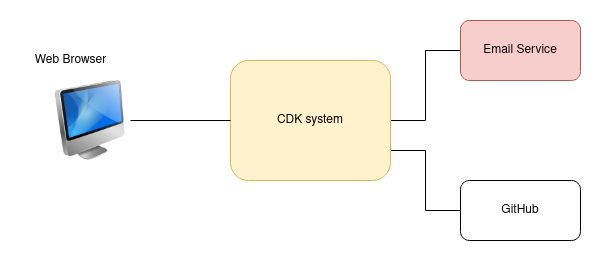
\includegraphics[width=1\linewidth]{misc/overviewDiagram.png}
    \caption{High Level View Diagram}
    \label{fig:enter-label}
\end{figure}

\newpage

\section{Component View}

The component diagram shows all the identified components and their interactions. We provide two different diagrams: 
\begin{itemize}
    \item In the first one we show how the various microservices interact with each other
    \item In the second one we show how the microservices interact with the external world.
\end{itemize}

After the diagrams a brief description of all the components will follow.

\subsection{Component Diagram}

\subsubsection{System Interaction}

\begin{figure}[H]
    \centering
    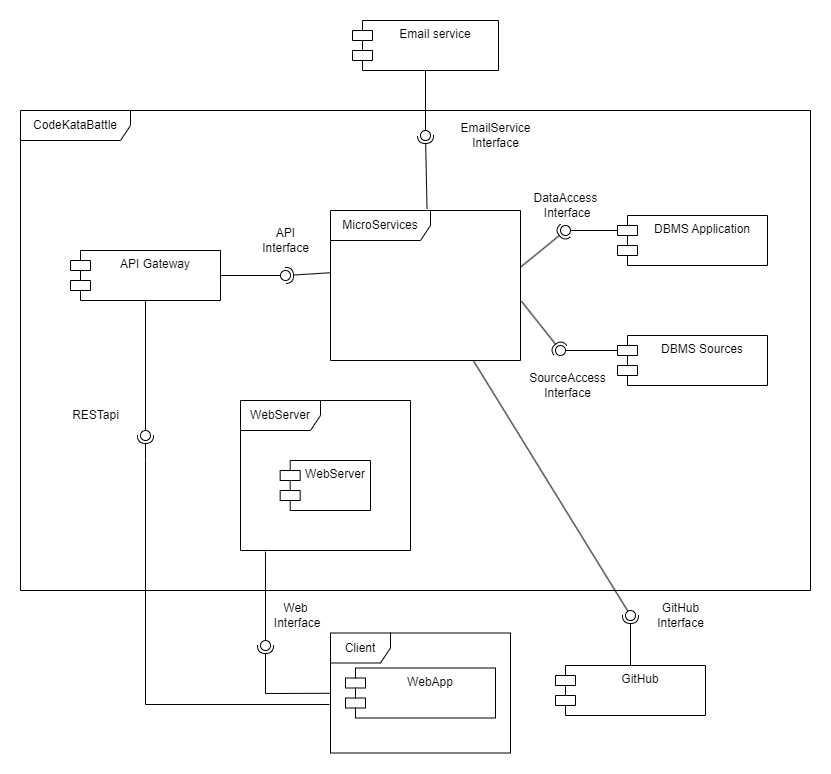
\includegraphics[width=1\linewidth]{misc//Images/Component.png}
    \caption{\ac{CKB} component diagram}
    \label{fig:enter-label}
\end{figure}

\subsubsection{Microservices Interaction}

\begin{figure}[H]
    \centering
    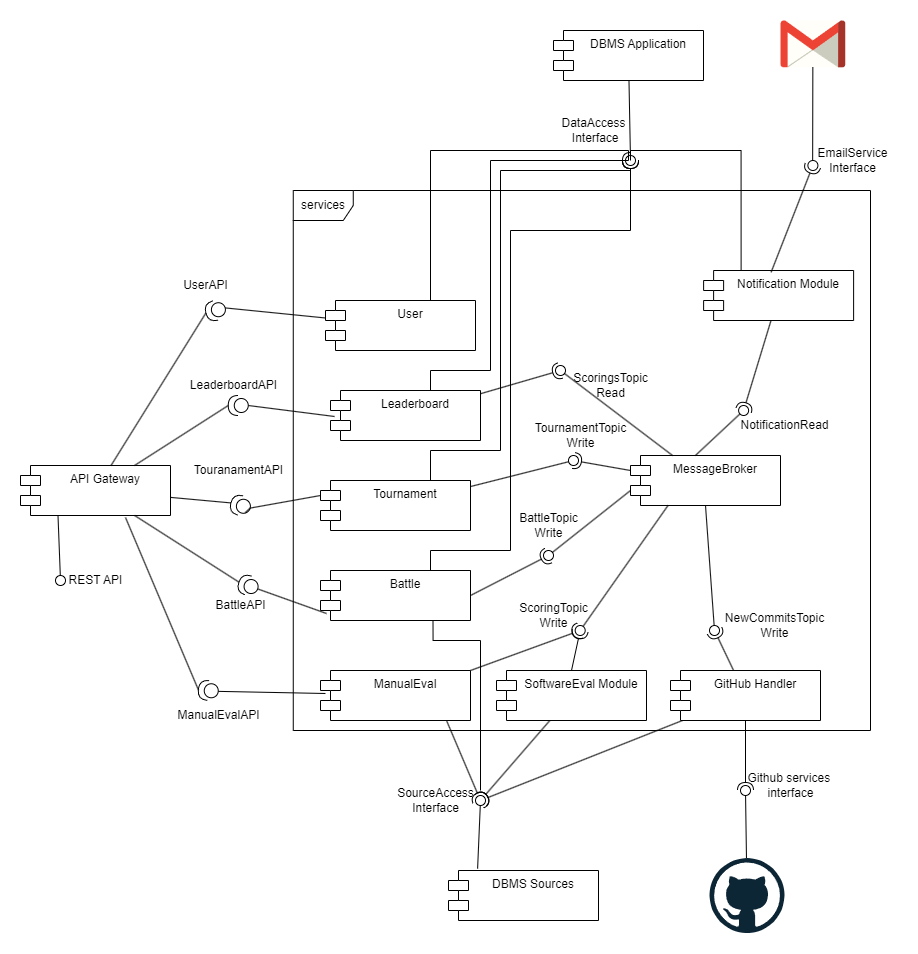
\includegraphics[width=1\linewidth]{misc//Images/microservicesComponentDiagram.png}
    \caption{\ac{CKB} Microservices Interactions}
    \label{fig:enter-label}
\end{figure}

\subsection{Components description}

The components are: 
\begin{itemize}
    \item GitHub handler :    Interfaces with GitHub APIs in order to: 
    \begin{itemize}
        \item create a Repository for a Battle after the subscription deadline
        \item retrieve the source code from a group after any commit and store it on a DataBase so that it can be automatically evaluated and then manually evaluated if needed during the consolidation phase
    \end{itemize}
\item Message broker :  It is the component tasked with dealing with messages from other services to enstablish the event based comunication between services. It keeps message queues for the various topics which some services produce and other are subscribe to
\item Email service :   Its is a third party service, used to send users various notifications.
\item User service: this component handles all the login and registration logic but not the authentication one.
\item API gateway : It handles client access to the various system services, it also handles the authorization aspects of the services use, to ensure system security.
\item Web server : It interfaces with the client browser and responds to its requests with the needed web pages(html+css+js).
\item WebApp : The part of the application that runs on the client browser. It is made of a set of web pages which are able to make requests to the web server and the services the system provides.
\item Github : It is the third party application that handles the battle repositories. 
\begin{itemize}
    \item The student users use its services outside the \ac{CKB} scope to fork a \ac{CK} assignement and work on its solution.
    \item The \ac{CKB} system interfaces with some Github services in order to create the repository and retrieve the solutions committed by students for evaluation.
\end{itemize}
\item DBMS (Application) : It is the DBMS that provides access to the database containting all the information about users, tournaments, battles and the scoring.
\item DBMS (Sources) : The DBMS for the database that keeps the source code related to any groups in any battles. This database is separated from the other in order to :
\begin{itemize}
    \item Optimize its performance , since the dimension of its records can be possibly way bigger.
    \item Have better control on the source codes to be stored, since they will run inside the \ac{CKB} system for evaluation, making it a security concern.
\end{itemize}
\item Tournament Service: The tournament service handles all aspects of a tournament, from the creation to the joining of students.
\item Battle Service: The battle service handles all aspects of a battle,  from the creation to the joining of students.
\item Notification Service: The notification Service handles all the user notifications. Students and Educators are gonna get email notification from this service whenever: a new tournament is created, a new battle is created, a final rank for a battle is available and a final battle for a tournament is available.
\item Leaderboard Service: The service handles all kinds of leaderboards present in the system. It exchanges messages with ManualEval and SoftwareEval and through those it updates the leaderboards of battles and tournaments inside the Application DBMS.
\item ManualEval Service: The component handles the consolidation stage of a battle(if it was required). It gives access to a group's sources in order to add a new score for the battle the group is participating.
\item SoftwareEval Service: The component handles the automatic scoring of new commits to the group's repository. Whenever a student commits to the repository GitHub sends a notification to the GithubHandler service which downloads the sources and signals to this component the neediness of an Evaluation
\end{itemize}
\newpage
\section{Deployment view}

The following deployment diagram shows how all the components are distributed and how they interact with each other.

\begin{figure}[H]
    \centering
    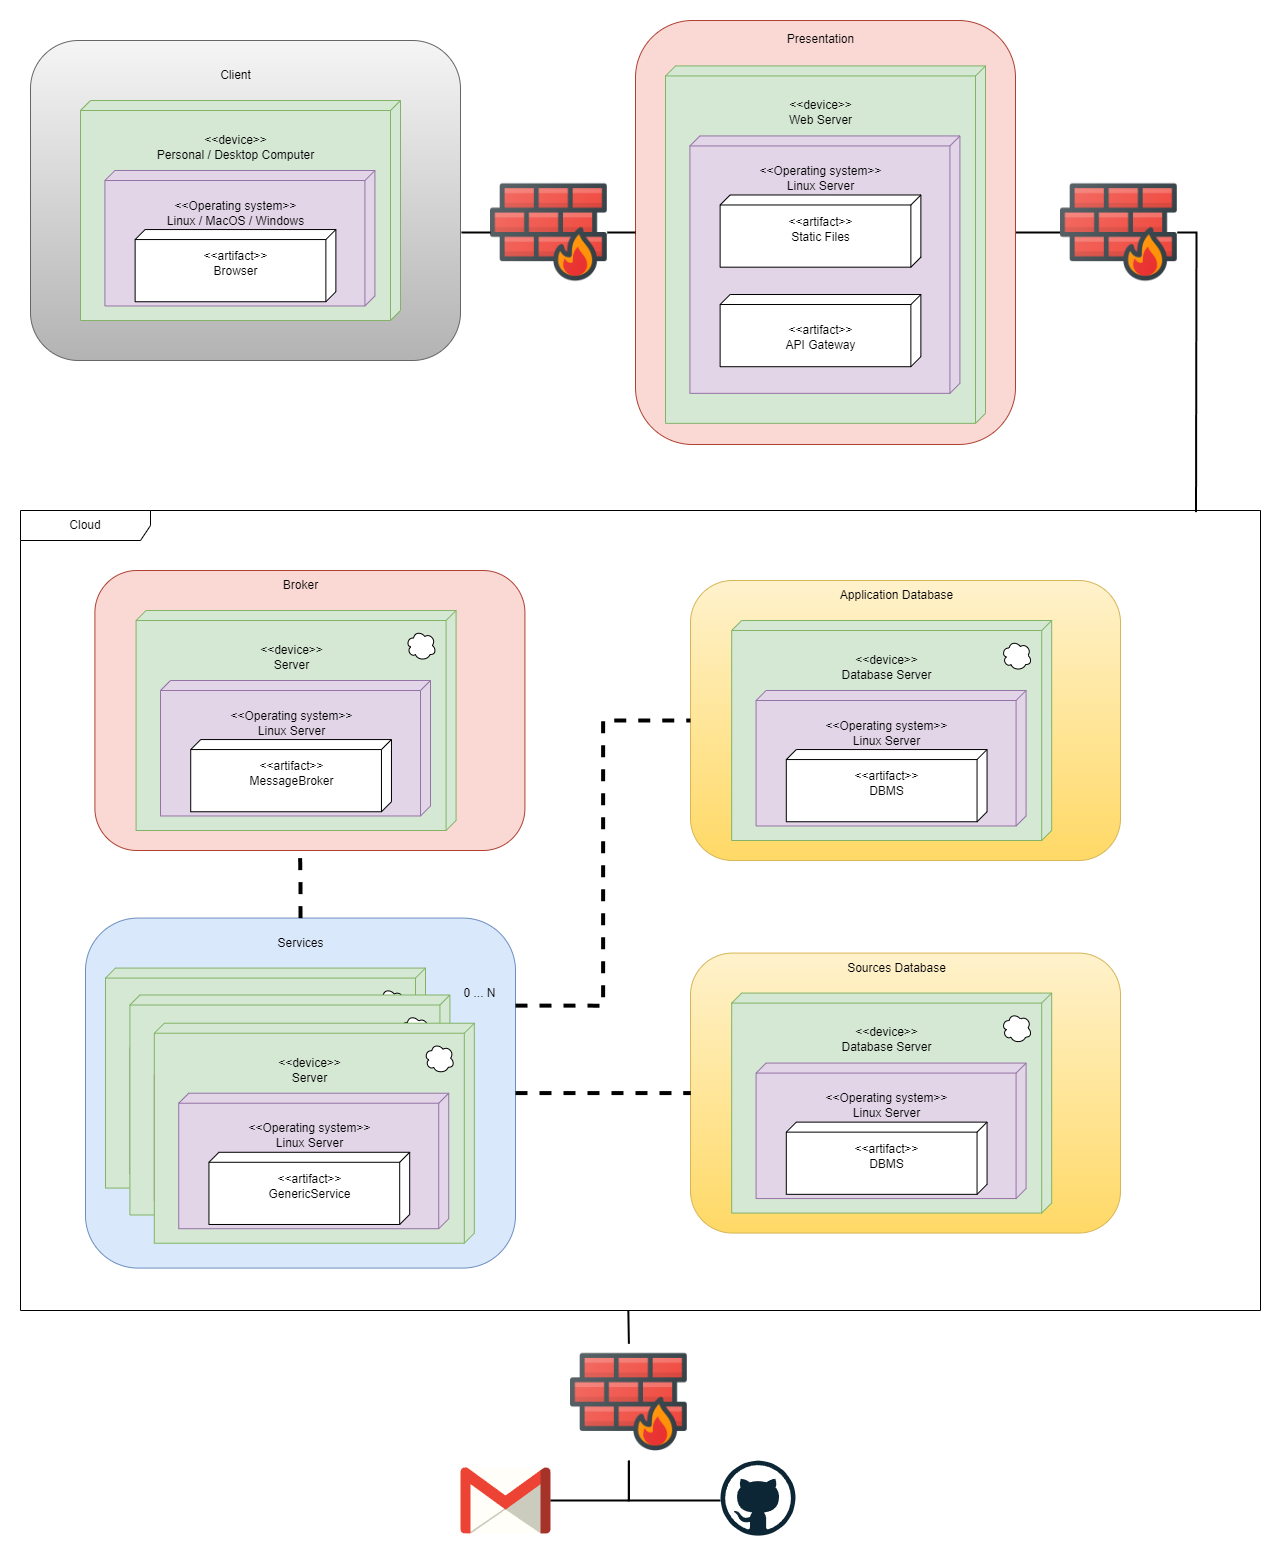
\includegraphics[width=1\linewidth]{misc//Images/Deployment.png}
    \caption{\ac{CKB} Deployement diagram}
    \label{fig:enter-label}
\end{figure}

\section{Runtime view}

Here we present the dynamics of our system through the use of sequence diagrams. All the interaction that use REST APIs start with the client request to an API that may contain a number of parameters, which are listed in the interface description of the API in the apposite document section, and end with either a positive response, eventually containing requested data and/or hyperlink for contextual page navigation (following REST's HATEOAS principle), or a negative response in case of any error.
For reading simplicity only positive responses are shown in the diagrams, as any other error response sent to the client always results in an error alert in the client application page.
In the interactions where the notification service is involved an email containing a message for the users is sent. The message content and destination is in the diagram description.
In some complex diagrams where the message broker is involved, a more specific description of its interaction with the other services is provided.

\subsection{Sign Up}

After the user has signed up, the positive REST response contains the hypertext to redirect the client to the tournament's main page.

\begin{figure}[H]
    \centering
    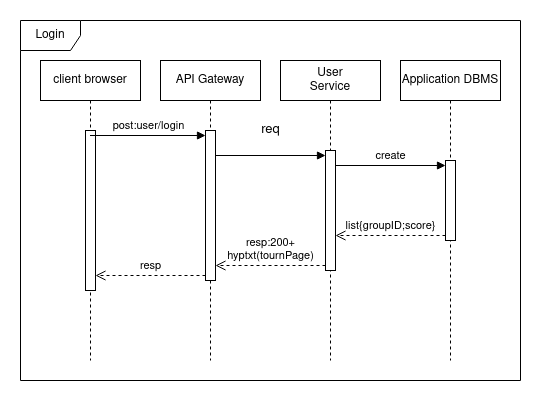
\includegraphics[width=1\linewidth]{misc//Images//UC/UC2.png}
    \caption{Sign up sequence diagram}
    \label{fig:enter-label}
\end{figure}
\newpage
\subsection{Sign In}

After the user has signed in, the positive rest response contains the hypertext to redirect the client to the tournaments main page.

\begin{figure}[H]
    \centering
    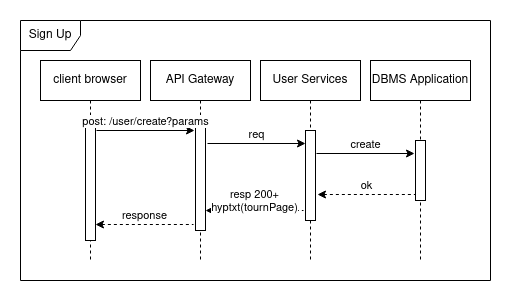
\includegraphics[width=1\linewidth]{misc//Images//UC/UC1.png}
    \caption{Sign in sequence diagram}
    \label{fig:enter-label}
\end{figure}
\newpage
\subsection{Create Tournament}

Once the tournament has been created, the client is redirected to the new tournament page and an email is sent to all CDK student users notifying them of the new tournament existence.

\begin{figure}[H]
    \centering
    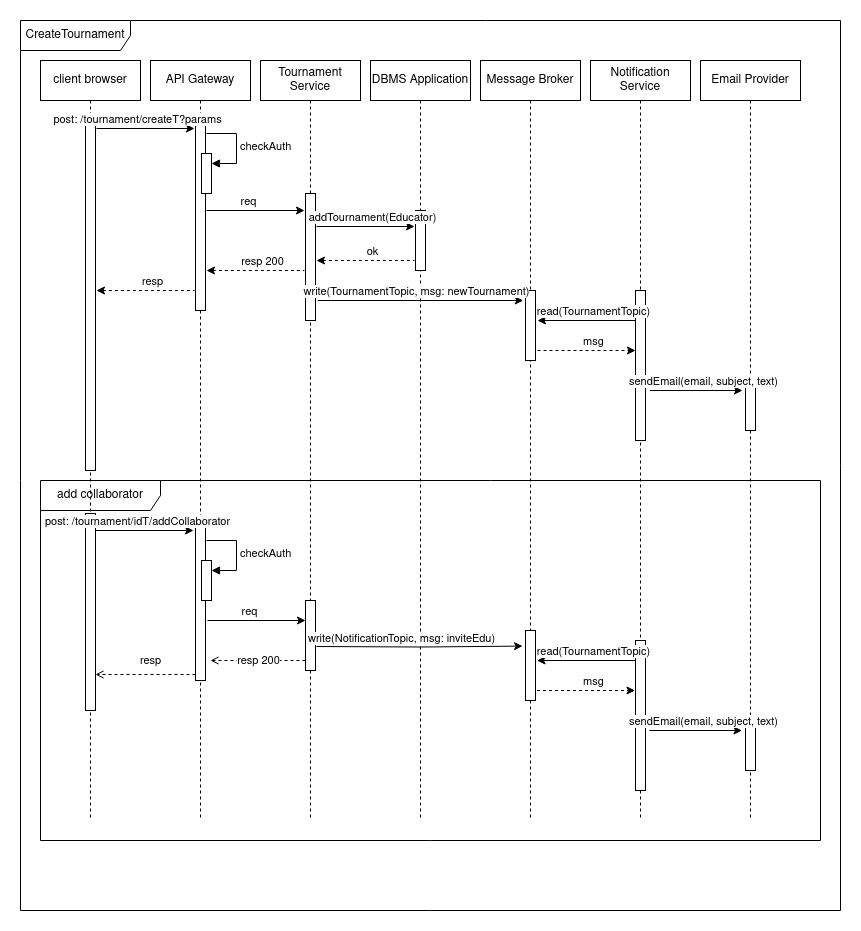
\includegraphics[width=1\linewidth]{misc//Images//UC/UC3.png}
    \caption{Create Tournament sequence diagram}
    \label{fig:enter-label}
\end{figure}
\newpage
\subsection{Subscribe To Tournament}

\begin{figure}[H]
    \centering
    \includegraphics[width=1\linewidth]{misc//Images//UC/UC4.png}
    \caption{Subscribe To Tournament sequence diagram}
    \label{fig:enter-label}
\end{figure}
\newpage
\subsection{Create Battle}

At the end of the interaction the systems response contains the hyperlink to the newly created battle resource. An email is also sent to all the student users that are subscribed to the tournament, notifying them of the new available battle.

\begin{figure}[H]
    \centering
    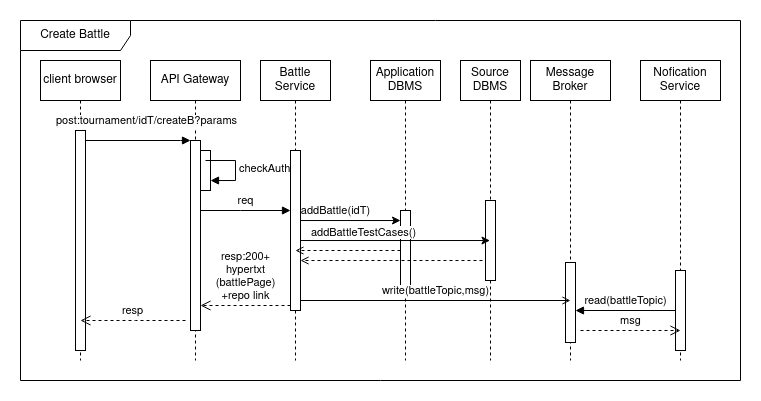
\includegraphics[width=1\linewidth]{misc//Images//UC/UC5.png}
    \caption{Create Battle sequence diagram}
    \label{fig:enter-label}
\end{figure}
\newpage
\subsection{Create Repository}

\begin{figure}[H]
    \centering
    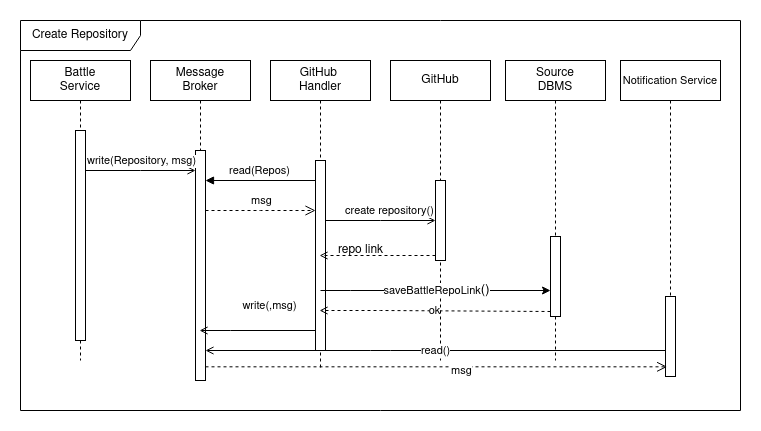
\includegraphics[width=1\linewidth]{misc//Images//UC/UC6.png}
    \caption{Create Repository sequence diagram}
    \label{fig:enter-label}
\end{figure}
\newpage
\subsection{Join Battle}

During the interaction the notification service sends an email the student listed from the user when joining the battle, notifying them of their position as group members in the battle.
If the battle group rules allows it and the user decide to join alone, the notification service won't read any message from the message broker, and no email will be sent.

\begin{figure}[H]
    \centering
    \includegraphics[width=1\linewidth]{misc//Images//UC/UC7.png}
    \caption{Join Battle sequence diagram}
    \label{fig:enter-label}
\end{figure}
\newpage
\subsection{Score Commit}

The interaction starts from GitHub notifying the system. Once the source code has been pulled it is stored in the source DBMS and a message notifying the new sources is sent to the message broker.
The software evaluation service is subscribed to the source topic and sees the notification, therefore it reads the sources from the source DBMS and starts to score the source code. Then it notifies the Leaderboard service with the new score through the message broker, which stores it as the group score in the application DBMS.

\begin{figure}[H]
    \centering
    \includegraphics[width=1\linewidth]{misc//Images//UC/UC8.png}
    \caption{Score Commit sequence diagram}
    \label{fig:enter-label}
\end{figure}
\newpage
\subsection{View Battle Ranking}

The response received from the client contains the Battle Leaderboard data which will be visualized.

\begin{figure}[H]
    \centering
    \includegraphics[width=1\linewidth]{misc//Images//UC/UC9.png}
    \caption{View Battle Ranking sequence diagram}
    \label{fig:enter-label}
\end{figure}
\newpage
\subsection{Manual Evaluation}

\begin{figure}[H]
    \centering
    \includegraphics[width=1\linewidth]{misc//Images//UC/UC10.png}
    \caption{Manual Evaluation sequence diagram}
    \label{fig:enter-label}
\end{figure}
\newpage
\subsection{Look at Tournament Leaderboard}

The response received from the client contains the Tournament Leaderboard data which will be visualized.

\begin{figure}[H]
    \centering
    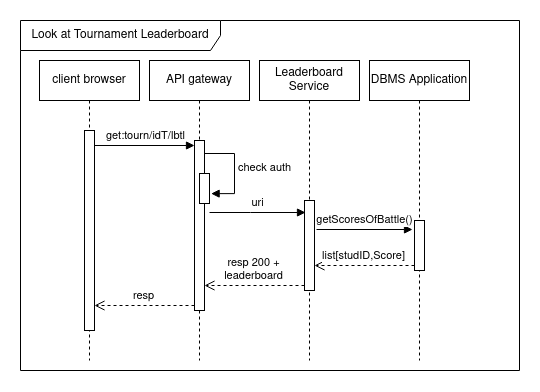
\includegraphics[width=1\linewidth]{misc//Images//UC/UC11.png}
    \caption{Look at Tournament Ranks sequence diagram}
    \label{fig:enter-label}
\end{figure}
\newpage
\subsection{Close Tournament}

\begin{figure}[H]
    \centering
    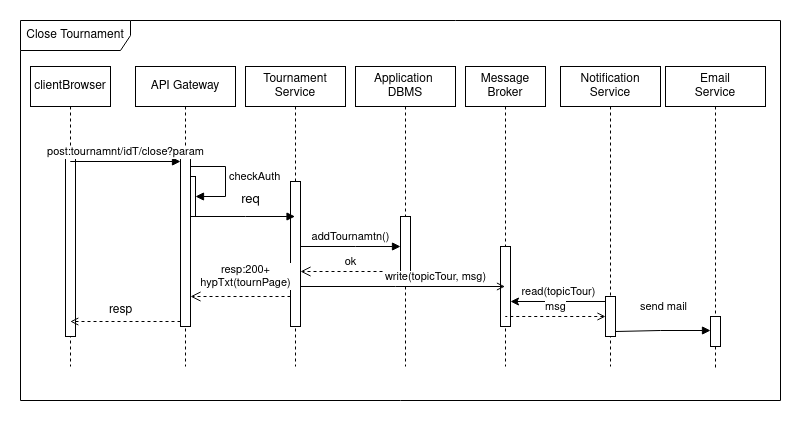
\includegraphics[width=1\linewidth]{misc//Images//UC/UC12.png}
    \caption{Close Tournament sequence diagram}
    \label{fig:enter-label}
\end{figure}
\newpage
\section{Component interfaces}

\subsection{Message Broker API}
The message broker exposes two methods:
\begin{itemize}
    \item read(Topic: int): Message: String
    \item write(Topic: int, Message: String)
\end{itemize}
All the microservices write/read on a particular topic exchanging JSON strings:



\begin{table}[h]
\hspace*{-4cm}
    \begin{tabular}{|c|c|c|c|}
    \hline
        \textbf{Topic} & \textbf{Publisher} & \textbf{Subscriber} & Content\\
    \hline
        Tournaments & Tournament Service & Notification Service & int: TournamentID, \\
         & & & bool: TournamentStatus \\
    \hline
        Battles & Battle Service & Notification Service & int BattleID,\\
        & & & int: BattleStatus \\
    \hline
        InvitationsBattle & Battle Service & Notification Service & int: groupID,\\
        & & & list[]: userID \\
    \hline
        InvitationsTournamet & Tournament Service & Notification Service & int: userID\\
        & & & int: TournamentID \\
    \hline
        Commits & GitHubHandler & SoftwareEval Service & int: groupID\\
    \hline
        Scores & ManualEval Service, SoftwareEval Service & Leaderboard Service & int: groupID\\
        & & & int: Score \\
    \hline
        Repository & Battle Service & GitHubHandler & int: battleID\\
    \hline
        RepoLinks & GithubHandler & Notification Service & int: battleID\\
        & & & String: LinkToRepository \\
    \hline
    \end{tabular}
    \hspace*{-4cm}
    \caption{Topics table}
    \label{tab:my_label}
\end{table}



\subsection{DBMS API}
\subsubsection{Data Access Interface}
Exposed by Application DBMS, used by Leaderboard, tournament, battle, group and user services. 
\begin{itemize}
    \item getSubscribedStudents(String : IDT): list[string studentID]
\end{itemize}
\paragraph{Used by Leaderboard Service}
\begin{itemize}
    \item getScoresOfTournament(String : IDT): Map[string: studenID; int: score]
    \item setScoresUserTournament(String:IDStud, String : IDT, int :score): void
    \item setScoresGroupBattle(String:IDGroup, String : IDB, int :score): void
    \item getScoresOfBattle(String: IDB): Map[ string: groupID, int: score]
\end{itemize}
\paragraph{Used by Notification Service}
\begin{itemize}
    \item getAllSignedStudent(): list[ string studID]
    \item getSubscribedStudent(string IDT): list[ string studID]
    \item getGroups(string IDB): map[string groupID; list[string studID]]
    \item getInvolvedEDUBattle(string IDB): list[ string eduID]
\end{itemize}
\paragraph{Used by Tournament Service}
\begin{itemize}
    \item addTournament(String : EduCreator):void
    \item grantBattleCreation(string : IDT, string : grantedEDU): void
    \item getCurrentTournamtn(): list[ string :tournamentID]
    \item getBattlesOfTourn(String : IDT):list[ string :battleID]
    \item checkEducatorPermission(String : IDT, String: IDEDU ): boolean response
\end{itemize}
\paragraph{Used by Battle Service}
\begin{itemize}
    \item getDeadlinesBattle(String: IDB): tuple(subsDL; submDL)
    \item addBattle(String TournamentID, string assignment,  int submDL, int subsDL, int maxsize, int minsize): string IDB
    \item getBattleAssignement(string IDB):  string assignment
    \item getBattleGroupRules(string IDB):  tuple(int  maxsize,int  minsize)
    \item getBattleAssignement(string IDB):  string assignment
    \item getBattleDeadlines(string IDB):  tuple(string submDL,string  subsDL)
    \item addGroup(list[string studID], String IDB): void
\end{itemize}
\paragraph{Used by User Service}
\begin{itemize}
    \item addStudent(String: UserName): void
    \item addEducator(String UserName): void
\end{itemize}
\subsubsection{Source Access Interface}
Exposed by Source DBMS, used by ManualEval, SoftwareEval, GithubHandler, Battle Service

\begin{itemize}
    \item addBattleTestCases(string IDB,list[ string] testcase):void
    \item getGroupSource(String: groupID, String: battleID): string SourceCodetxt
    \item saveGroupSource(String: groupID, String: battleID, String: SourceCodetxt): void
\end{itemize}
\subsection{RESTful API}
These are all external API's exposed by the API Gateway and used by the client application. They follow rest principle, each service handles some resources revolving around a particular aspect of the application i.e.: battles, tournaments, etc.  
Here follows a three of the uri path tree of the exposed resources:  
 
\begin{figure}[H]
    \centering
    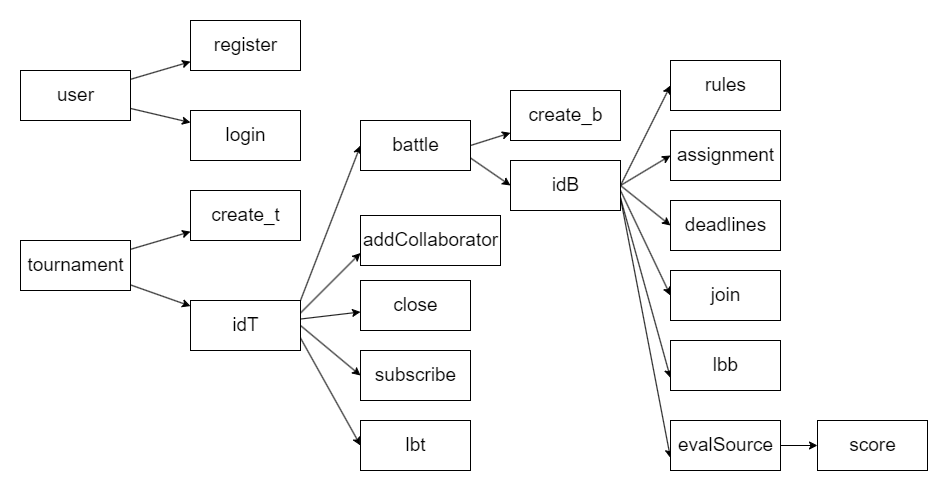
\includegraphics[width=1\linewidth]{misc//Images/RESTresources.png}
    \caption{Resource Tree path}
    \label{fig:enter-label}
\end{figure}
\subsubsection{UserAPI}

\begin{itemize}
\item \textbf{POST /user/register}\newline  
registerUser(StringU:UserName, String : UserType):void
\item \textbf{POST /user/login}\newline  
login(String : psw, String : UserID):void
\end{itemize}
\subsubsection{TournamentAPI}
\begin{itemize}
    \item \textbf{GET /tournament/}\newline  
    getCurrentTournament(String: UserId,String: UserType) : list$<$Tournament$>$
    \item \textbf{POST /tournament/create\_t}\newline  
    createTournament(String: UserId,String: UserType, String : TournamentName): void  
    \item \textbf{POST /tournament/{idT}/addCollaborator}\newline   
    addCollaborator(String: UserId,String: UserType, String : CollaboratorID):void  
    \item \textbf{POST /tournament/{idT}/close}\newline  
    closeTournament(String: UserId,String: UserType, String : TournamentID): void 
    \item  \textbf{POST /tournament/{idT}/subscribe}\newline  
    subscribeTournament(String: UserId,String: UserType, String : TournamentID) : void
    \item \textbf{GET /tournament/{idT}/battle/}\newline  
    getTournamentsBattles(String: UserId,String: UserType, String : TournamentID): List$<$Battle$>$  
\end{itemize}

\subsubsection{BattleAPI}
\begin{itemize}
    \item \textbf{POST /tournament/{idT}/battle/create\_b}\newline    
    createBattle(String: UserId,String: UserType, String : BattleName, tuple(int maxsize, int minsize): groupRule, string : assignemtent, tuple(date: subs, date: subm): deadline, list[ string]: testcases): void  
    \item \textbf{GET /tournament/{idT}/battle/{idB}/rules}\newline
     getGroupRules(String: UserId, String : BattleID): Tuple (int :MaxSize, int: MinSize)  
    \item \textbf{GET /tournament/{idT}/battle/{idB}/assignment}\newline  
     getAssignemntText(String: UserId, String : BattleId): String AssignmentText  
    \item \textbf{GET /tournament/{idT}/battle/{idB}/deadlines}\newline  
     getDeadlines(String: UserId, String : BattleID):Tuple (int :SubscriptionDL, int: SubmissionDL)  
    \item \textbf{POST /tournament/{idT}/battle/{idB}/join}\newline  
    joinBattle( String: UserId, String : BattleID, String: UserType, OPTIONAL List$<$ StudentID$>$ ): void
\end{itemize}

\subsubsection{LeaderBoardAPI}

\begin{itemize}
    \item \textbf{GET /tournament/{idT}/lbt}  \newline
    getLeaderBoardTournament(): LeaderBoard
    \item \textbf{GET /tournament/{idT}/battle/{idB}/lbb}  \newline
    getLeaderBoardBattle():Leaderboard  
\end{itemize}
\subsubsection{ManualEvaluationAPI}

\begin{itemize}
    \item \textbf{GET /tournament/{idT}/battle/evalSource}\newline
    getSourcesForEval(String: UserId, String : BattleID, String: UserType ): String SourceCode
    \item \textbf{POST /tournament/{idT}/battle/evalSource/score}\newline
    addManualScore(String: UserId, String : BattleID, String: UserType, int : score)
    : void
\end{itemize}
\section{Selected architectural styles and patterns}

\subsection{Microservices}

A microservice architecture is needed mainly in order to freely scale some component indipendently from others, like the \textbf{software evaluation} service, which at time may need much more computational resources, meanwhile other services are less likely to require as much, as they don't perform heavy activities like code analysis and execution.
Other then that, this style of architecture provides many more general advantages, making easy to choose. 

\subsubsection{API Gateway}

The API gateway provvides many benefits as the only entry point between the client and services.
Here are the ones which were more valued: Security and authentication; Load balancing; Caching. 

\subsection{Hybrid architecture (REST and EBA)}

\subsubsection{Event Based architecture}

Used in the system backend for the communication between microservices.  
The use of aynchronous communication allows for more flexibility and scalability, both important for some of the microservices, in particular the \textbf{software evaluation} service, which needs to scale indipndently from other services becaus of its higher computational needs.
Moreover the the system interfaces with Guthub APIs which have also an EBA.

\subsubsection{Rest(ful APIs)}

The services wich provide functionalities for the front end expose RESTful APIs.  
This way there is a greater separation of concern between front end and backend, as when developing the client application a team doesnt need to concern themeself with the internal structure of the system made of services, but only need to know the URI tree path used to access resources and their operations.

\section{Other design decisions}

There were no other design decisions to note.
\newpage

\chapter{User Interface Design}
In this section will be presented an overview of the user's interface of the \ac{CKB} system. The application, as previously discussed will be a web app, accessible from a desktop browser. The access from mobile will be enabled and the interface will be scaled appropriately.

\section{General Overview}

The image below shows a map of the pages accessible by Educators and Students.

\begin{figure}[H]
    \centering
    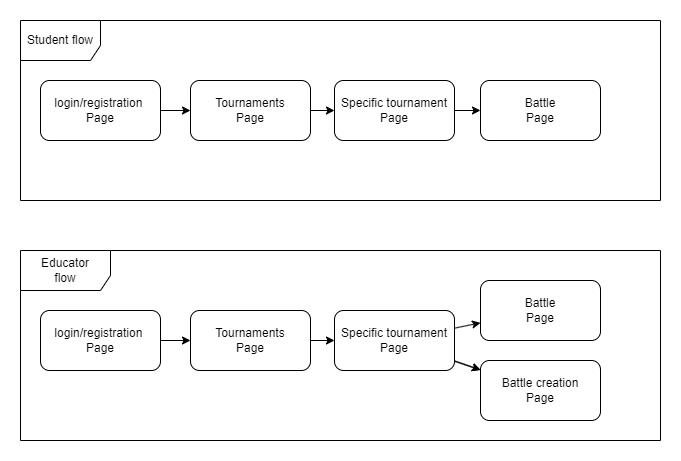
\includegraphics[width=0.95\linewidth]{misc//Images/flow.png}
    \caption{Web pages map}
    \label{fig:enter-label}
\end{figure}
\newpage
\subsubsection{Login Page}
This page is the first one viewed by the user when accessing the application. It contains two forms, one for the login of the user and one for the registration.
For the login the user can input their Username, password and select whether the user is an Educator or not.

For the registration the user is asked to insert their desired username, the password, and the type of user he desires to register as. Also the user has to insert the email where he will receive notification.

Once the user has created the account or logged into his own account he is directed to the tournaments page.

\begin{figure}[H]
    \centering
    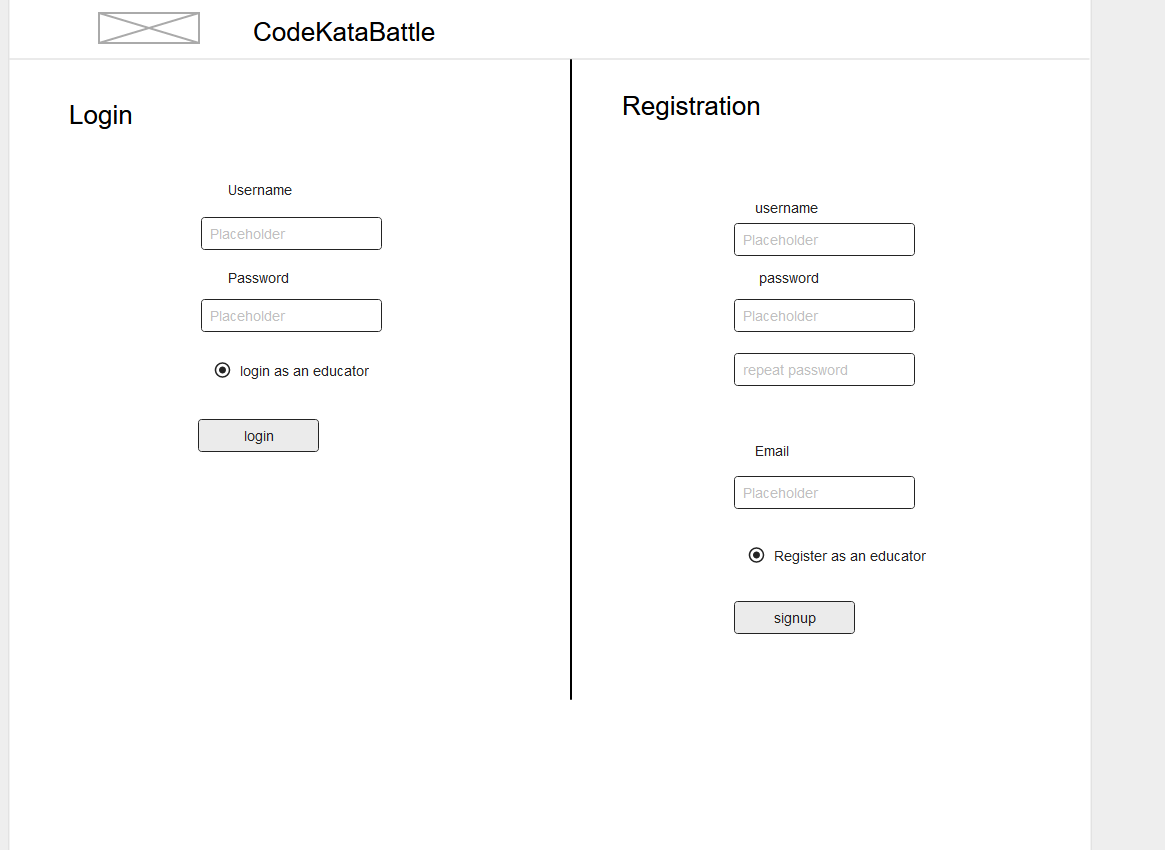
\includegraphics[width=1\linewidth]{misc//Images//UI Mockups/login.png}
    \caption{Login Page}
    \label{fig:enter-label}
\end{figure}
\newpage
\subsubsection{Main Page}
In this page a user can see the list of ongoing tournaments and the list of tournaments he/she is involved in, from which a specific tournament can be chosen to be redirected to.
If the user is an Educator then the page will also display a form for the creation of a tournament.

\begin{figure}[H]
    \centering
    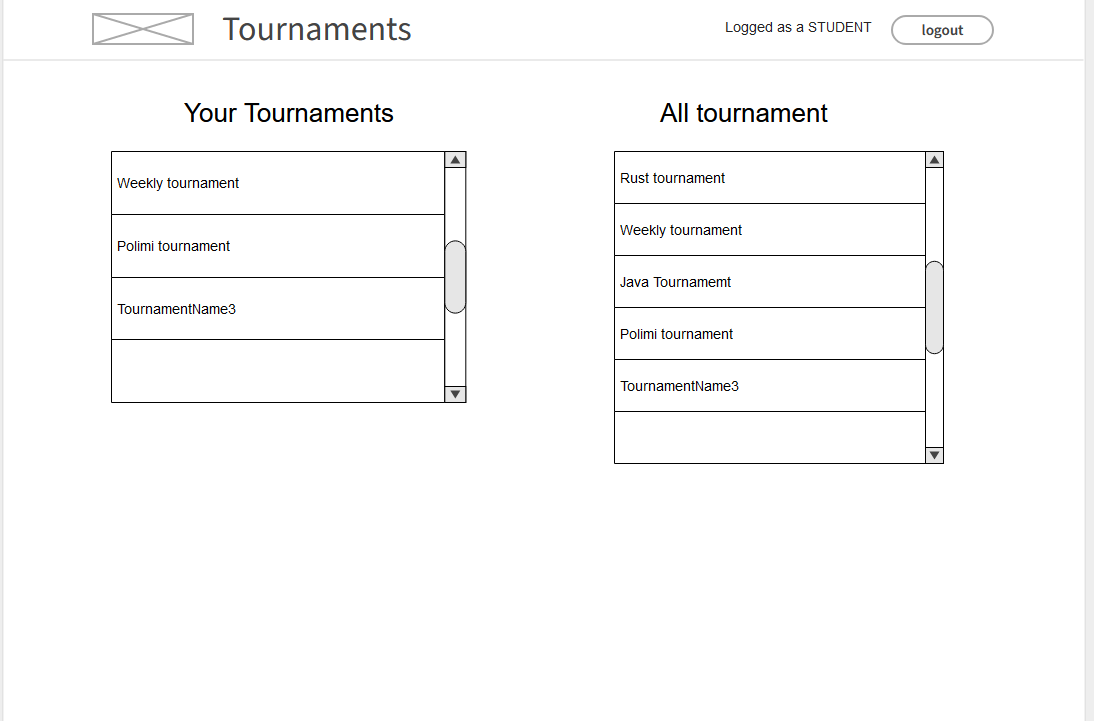
\includegraphics[width=0.8\linewidth]{misc//Images//UI Mockups/studMain.png}
    \caption{Student Main Page}
    \label{fig:enter-label}
\end{figure}


\begin{figure}[H]
    \centering
    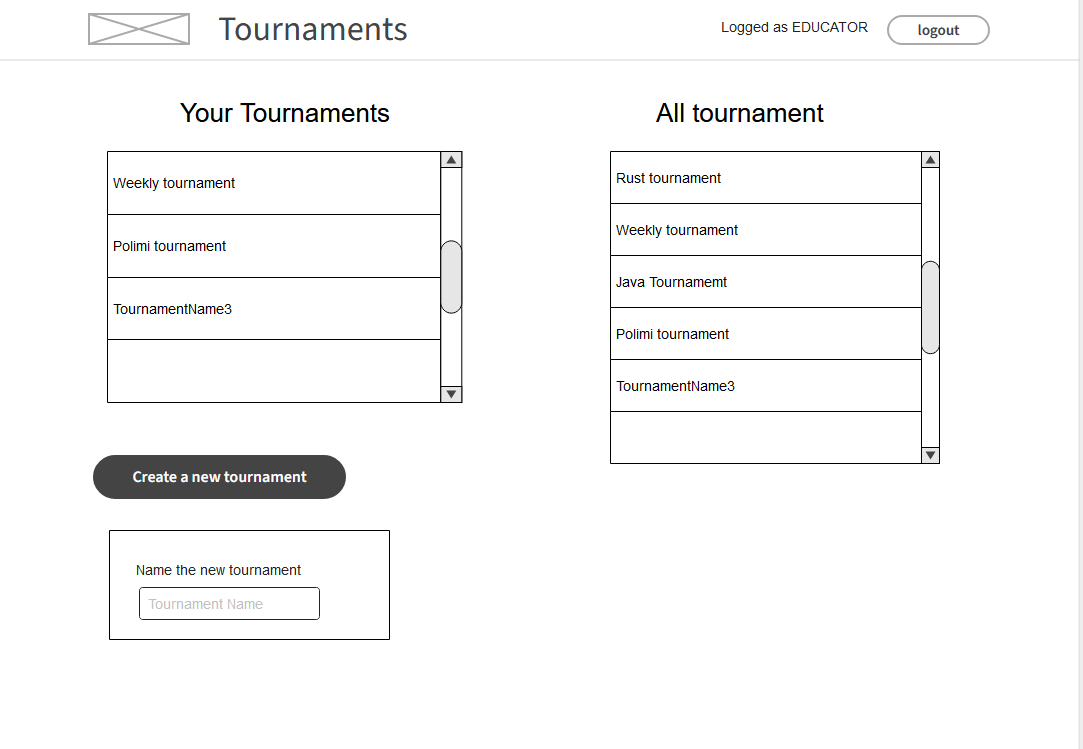
\includegraphics[width=0.8\linewidth]{misc//Images//UI Mockups/eduMain.png}
    \caption{Educator Main Page}
    \label{fig:enter-label}
\end{figure}

\newpage
\subsubsection{Tournament Page}
This page contains the list of battle in the context of the current tournament as well as the tournament leaderboard and 3 buttons.
The buttons allow the user to either create a battle in the tournament context, add a collaborator to the tournament or close the tournament.
The battles in the list can be selected to be directed to the selected battle page.
If the user is a student then instead of the three buttons there will be only one, allowing the student to join the tournament.

\begin{figure}[H]
    \centering
    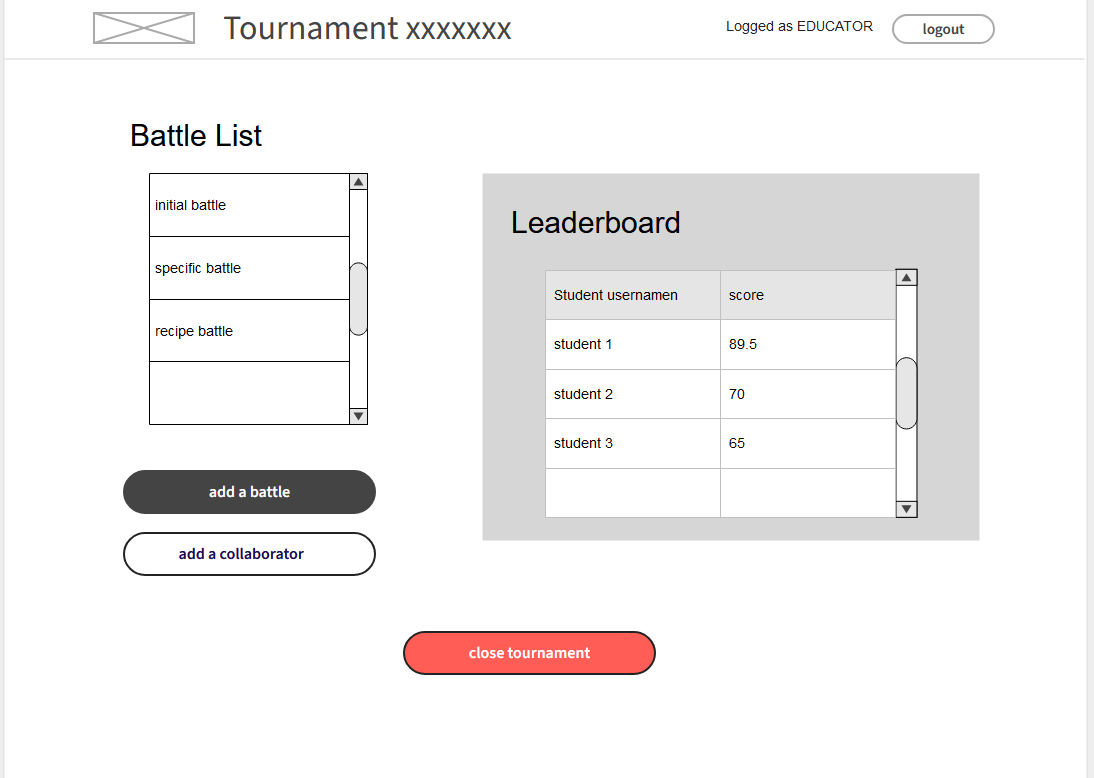
\includegraphics[width=0.7\linewidth]{misc//Images//UI Mockups/eduTournament.png}
    \caption{Educator Tournament Page}
    \label{fig:enter-label}
\end{figure}

\begin{figure}[H]
    \centering
    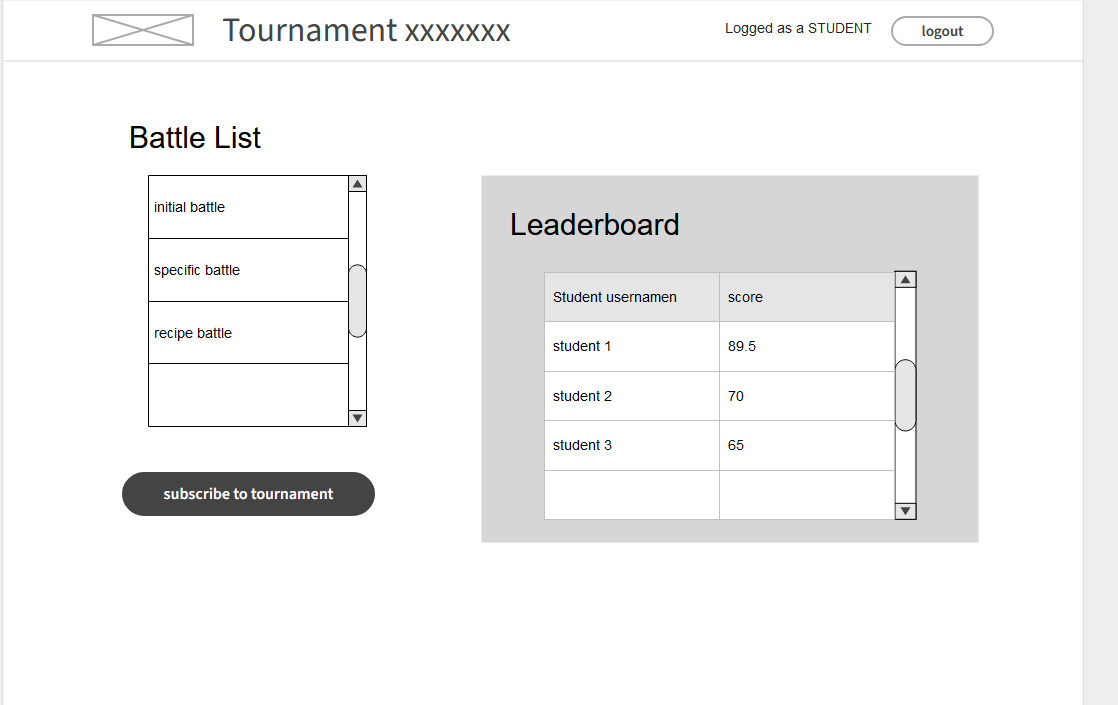
\includegraphics[width=0.7\linewidth]{misc//Images//UI Mockups/studTournament.png}
    \caption{Student Tournament Page}
    \label{fig:enter-label}
\end{figure}
\newpage
\subsubsection{Battle Creation Page}
The page presents a form where an educator can insert: 
\begin{itemize}
    \item Battle name;
    \item Text assignment for the \ac{CK}; 
    \item The two deadlines,
    \item The group rules.
\end{itemize}
There is also an upload form for the \ac{CK} testcases.

\begin{figure}[H]
    \centering
    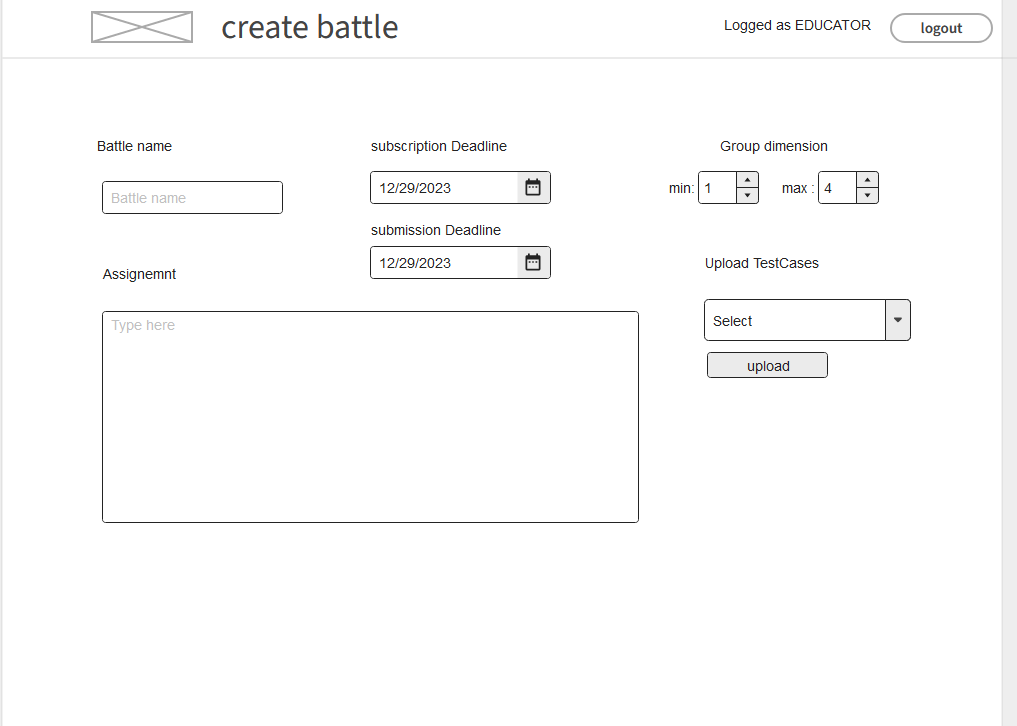
\includegraphics[width=1\linewidth]{misc//Images//UI Mockups/createBattle.png}
    \caption{Battle Creation}
    \label{fig:enter-label}
\end{figure}
\newpage
\subsubsection{Battle Page}
For both type of users the page presents the text of the assignment, the rules for the group size, the deadlines and finally the battle leaderboard.
In the student version during the battle subscription phase a button for joining the battle is present. When clicked the user is asked to insert a list of other student to join the battle with( following the group rules) in a form.

\begin{figure}[H]
    \centering
    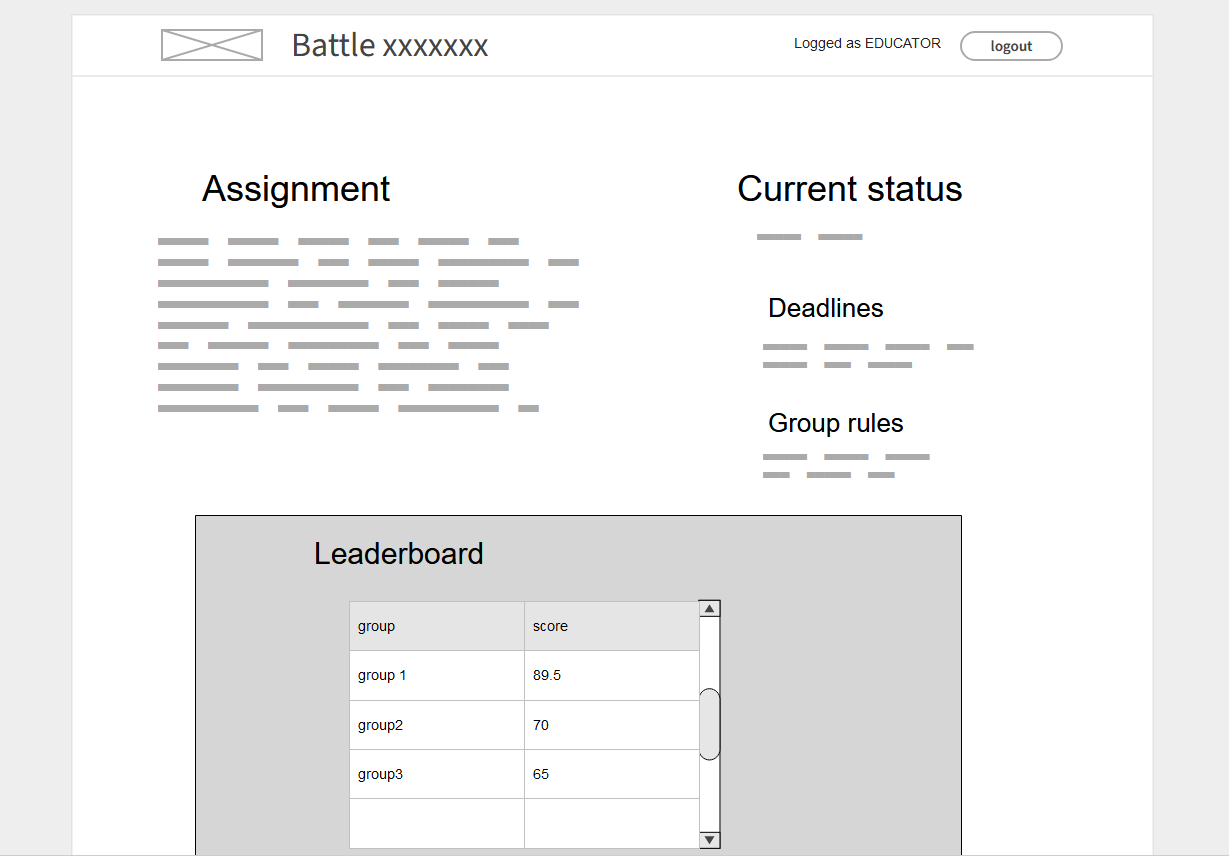
\includegraphics[width=1\linewidth]{misc//Images//UI Mockups/battle.png}
    \caption{Battle Page}
    \label{fig:enter-label}
\end{figure}
\newpage
\subsubsection{Manual Evaluation Page}

The page contains the source code of the group to be manually reviewed and an input where the user can put the decided score to be sent after clicking the 'score group' button.

\begin{figure}[H]
    \centering
    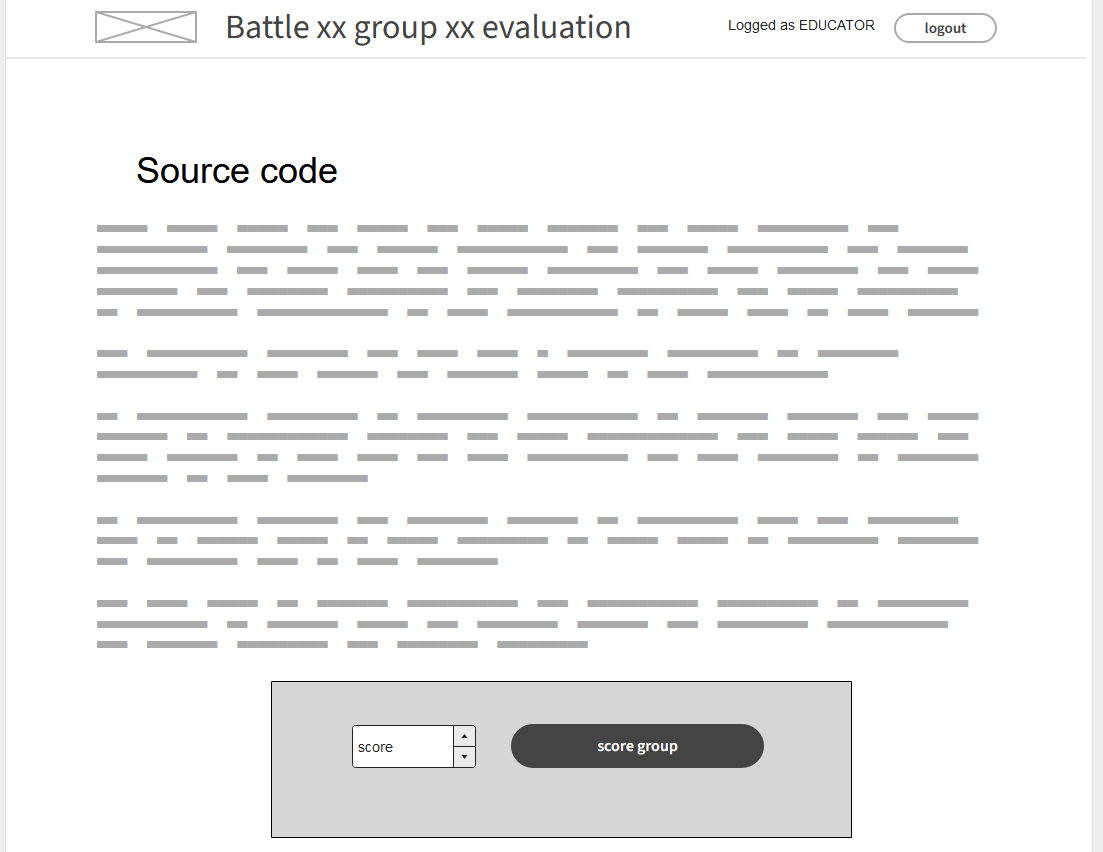
\includegraphics[width=1\linewidth]{misc//Images//UI Mockups/manualEval.png}
    \caption{Battle Page}
    \label{fig:enter-label}
\end{figure}
\newpage

\chapter{Requirements Traceability}
\section{External Interface Requirements}
\subsection{User Interfaces}
There are no user interface requirements.

\subsection{Hardware Interfaces}
There are no hardware interface requirements.

\subsection{Software Interfaces}
The \ac{CKB} system relies on the use of the GitHub system in order to manage the battle's repositories. With every new battle created a new repository is generated on Github. Every group of student will then fork this repository and setup a workflow in order to notify the \ac{CKB} system of every new commit through Github.

\subsection{Communication Interfacess}
There are no communication interface requirements.

\newpage
\section{Functional Requirements}
\subsection{Requirements}
The \ac{CKB} system offers several functionalities. In the following table we describe all the requirements that the system should respect in order to achieve its goals.
\begin{center}
    \begin{longtable}{ |l|p{0.85\linewidth}| }
        \hline
            \textbf{ID} & \textbf{Description}\\
        \hline
            R1 & The platform allows a signed in educator to create tournaments \\
        \hline
            R2 & Educators can create battles in the context of a specific tournament they are involved in (Either by creation or by invitation)  \\
        \hline
            R2.1 & The platform allows an educator that created a tournament, to invite other educator and to grant them permission to create battles in the tournament context \\
        \hline
            R2.2 & The platform allows an educator to upload the codekata (description and software project, including test cases and build automation scripts) when creating a battle \\
        \hline
            R2.3 & The platform allows an educator to set subscribtion and submission deadlines when creating a battle \\
        \hline
            R2.4 & The platform allows an educator to set minimum and maximum group size when creating a battle \\
        \hline
            R2.5 & The platform allows an educator creating a battle to include a manual evaluation stage \\
        \hline
            R3 & The platform allows students to subscribe to a tournament \\
        \hline
            R4 & The platform allows a student subscribed to a tournament to join a battle in that tournament context \\
        \hline
            R4.1 & The platform allows students to create a group by inviting other students when joinin a battle \\
        \hline
            R5 & The platform allows Students to login \\
        \hline
            R6 & The platform allows Educators to login  \\
        \hline
            R7 & If manual evaluation is required during consolidation stage the platform allows an educator to go through sources and add a score to the group score \\
        \hline
            R8 & The platform allows all users to view student ranks from previous and current tournaments \\
        \hline
            R8.1 & For every tournament the platform maintains a ranking for students based on the sum of their battle scores \\
        \hline
            R9 & The platform pulls group sources from Github when it receives a notification within the submission deadline \\
        \hline
            R9.1 & The platform analyzes, runs testcases and scores the source of a group solution for a codekata battle and updates the group score accordingly \\
        \hline
            R10 & The platform allows all user to sign in \\
        \hline
            R11 & The platform allows educators to close tournaments  \\
        \hline
            R12 & When a battle deadline expires the platform sets the battle status to consolidation stage  \\
        \hline
            R13 & The platform allows all users who are involved in a battle to look at group ranks for that battle  \\
        \hline
            R13.1 & For every battle the platform maintains a ranking of the groups based on their battle score  \\
        \hline
            R14 & The platform will notify signed students of a newly created tournament  \\
        \hline
            R15 & The platform shall notify students who are subscribed into a tournament that a new battle is available in that tournament context  \\
        \hline
            R16 & The plaftorm shall notify students who are participating in a battle that the final rank for that battle is available  \\
        \hline
            R17 & The plaftorm shall notify students who are subscribed in a tournament that the final rank for that tournament is available  \\
        \hline
            R18 & The platform shall create a new repository with Github for every new battle in any tournament after the submission deadline expires\\
        \hline
            R19 & The platform shall send the battle repository link to students who joined that battle after the submission deadline expires\\
        \hline
    \end{longtable}
\end{center}
\subsection{Mapping on goals}

\begin{center}
    \begin{longtable}{|l|l|p{0.50\linewidth}|}
        \hline
            \textbf{Goal} & \textbf{Domain Assumption} & \textbf{Requirements} \\
        \hline
            G1 & A5, A6 & R1, R11, R6, R10\\
        \hline
            G2 & & R2, R2.1, R2.2, R2.3, R2.4, R2.5, R6, R10\\
        \hline
            G3 & & R3, R14, R5, R6, R10 \\
        \hline
            G4 & A1, A4 & R4, R4.1, R15, R5, R6, R10, R18, R19\\
        \hline
            G5 & A2, A3 & R7, R9, R9.1, R12, R5, R10\\
        \hline
            G6 & & R8, R8.1, R13, R13.1, R16, R17, R5, R6, R10\\
        \hline
    \end{longtable}
\end{center}

\subsubsection{An educator can manage a tournament}

\begin{itemize}
    \item R1: The platform allows a signed in educator to create tournaments
    \item R11: The platform allows an educator to close a tournament
    \item R6: The platform allows Educators to login
    \item R10: The platform allows all user to sign in
    \item A5: Educators will only close a tournament when no battle is still ongoing
    \item A6: Only the Educator who created the tournament will close it
\end{itemize}

\subsubsection{An educator can create battles inside of a tournament in which he is involved}

\begin{itemize}
    \item R2: Educators can create battles in the context of a specific tournament they are involved in (Either by creation or by invitation)
    \item R2.1: The platform allows an educator that created a tournament, to invite other educator and to grant them permission to create battles in the tournament context
    \item R2.2: The platform allows an educator to upload the codekata (description and software project, including test cases and build automation scripts) when creating a battle
    \item R2.3: The platform allows an educator to set subscribtion and submission deadlines when creating a battle
    \item R2.4: The platform allows an educator to set minimum and maximum group size when creating a battle
    \item R2.5: The platform allows an educator creating a battle to include a manual evaluation stage
    \item R6: The platform allows Educators to login
    \item R10: The platform allows all user to sign in
\end{itemize}

\subsubsection{Students can partecipate in tournaments created by an educator}

\begin{itemize}
    \item R3: The platform allows students to subscribe to a tournament
    \item R14: The platform will notify signed students of a newly created tournament
    \item R5: The platform allows Students to login
    \item R6: The platform allows Educators to login
    \item R10: The platform allows all user to sign in
\end{itemize}

\subsubsection{Students can partecipate in battles created by an educator, alone or in groups}

\begin{itemize}
    \item R4: The platform allows a student subscribed to a tournament to join a battle in that tournament context
    \item R4.1: The platform allows students to create a group by inviting other students when joinin a battle
    \item R15: The platform shall notify students who are subscribed into a tournament that a new battle is available in that tournament context
    \item R5: The platform allows Students to login
    \item R6: The platform allows Educators to login
    \item R10: The platform allows all user to sign in
    \item R18: The platform shall create a new repository with Github for every new battle in any tournament after the submission deadline expires
    \item R19: The platform shall send the battle repository link to students who joined that battle after the submission deadline expires
    \item A1: The students can correctly setup the Github actions workflow
    \item A4: Students are always able to create a group to join a battle
\end{itemize}

\subsubsection{Students are scored based on their performance in battles}

\begin{itemize}
    \item R7: If manual evaluation is required during consolidation stage the platform allows an educator to go through sources and add a score to the group score
    \item R9: The platform pulls group sources from Github when it receive a notification within the submission deadline
    \item R9.1: The platform analyzes, runs testcases and scores the source of a group solution for a codekata battle and updates the group score accordingly
    \item R12: When a battle deadline expires the platform sets the battle status to consolidation stage
    \item R5: The platform allows Students to login
    \item R10: The platform allows all user to sign in

    \item A2: An educator will complete the manual evaluation
    \item A3: Github will always notifies the CKB platform after every student commit
\end{itemize}

\subsubsection{The platform allows students and educators to compare the performance of students}

\begin{itemize}
    \item R8: The platform allows all users to view student ranks from previous and current tournaments
    \item R8.1: For every tournament the platform maintains a ranking for students based on the sum of their battle scores
    \item R13: The platform allows all users who are involved in a battle to look at group ranks for that battle
    \item R13.1: For every battle the platform maintains a ranking of the groups based on their battle score
    \item R16: The plaftorm shall notify students who are participating in a battle that the final rank for that battle is available
    \item R17: The plaftorm shall notify students who are subscribed in a tournament that the final rank for that tournament is available
    \item R5: The platform allows Students to login
    \item R6: The platform allows Educators to login
    \item R10: The platform allows all user to sign in
    
\end{itemize}

\subsection{Use Case Diagrams}

\subsubsection{Student Use Case Diagram}
\begin{figure}[H]
    \centering
    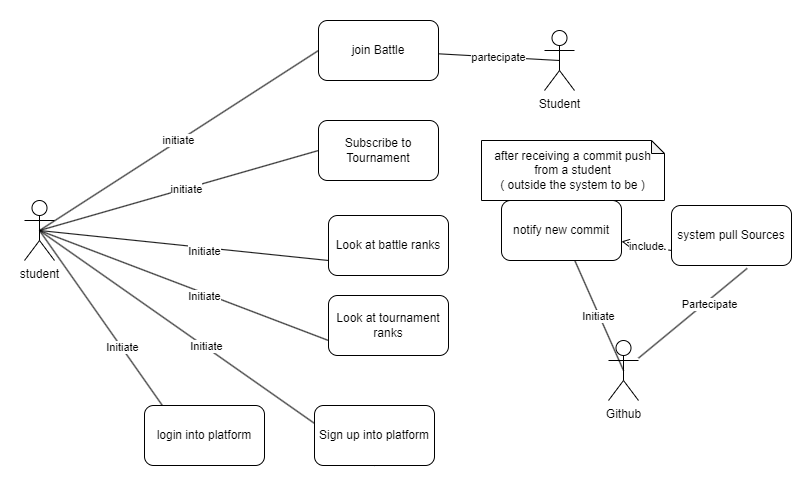
\includegraphics[width=1\linewidth]{misc//Images//UC/StudentScenarios.png}
    \caption{Student Use Case Diagram}
    \label{fig:enter-label}
\end{figure}


\subsubsection{Educator Use Case Diagram}
\begin{figure}[H]
    \centering
    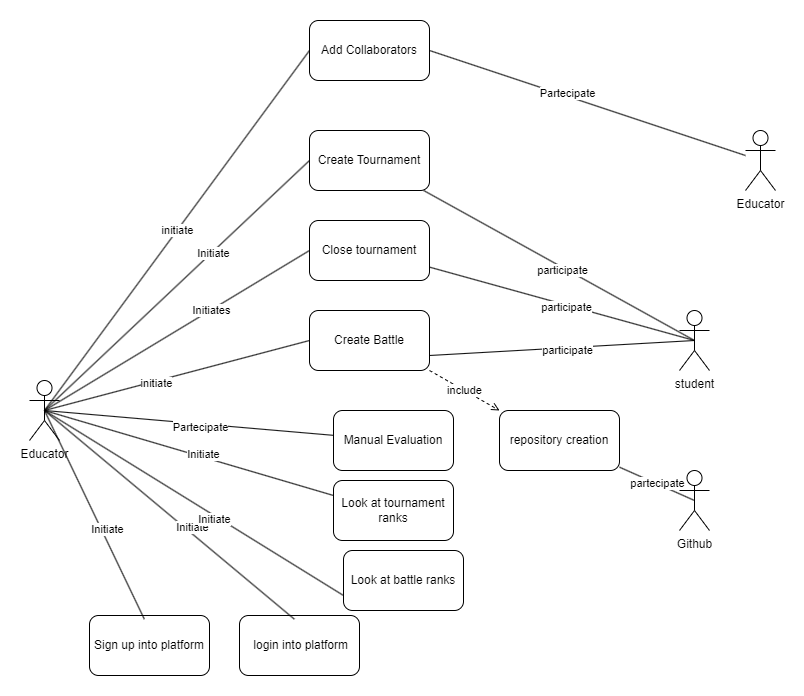
\includegraphics[width=1\linewidth]{misc//Images//UC/EducatorScenarios.png}
    \caption{Educator Use Case Diagram}
    \label{fig:enter-label}
\end{figure}

\subsection{Use Cases}
In this section we analyze the various use cases of the system by describing the actors, entry conditions, event flow, exit conditions and exceptions for all of them.

\newpage
\subsubsection{UC1: Sign Into Platform}
\begin{center}
    \begin{longtable}{lp{0.75\linewidth}}
        \hline
            Actor & Users(Educators, Students)\\
        \hline
            Entry condition & A user accesses the platform for the very first time\\
        \hline
            Event Flow & 1. User reaches the platform\\
                &2. User clicks on "sign in" button\\
                &3. User fills out own info and decides if they want to be an Educator or student\\
                &4. User concludes the registration by clicking "finish" button\\
        \hline
            Exit & User is successfully registered on the platform as either educator or student\\
        \hline
            Exception & Missing or wrong input by user during registration form\\
        \hline
    \end{longtable}
\end{center}


\begin{figure}[H]
    \centering
    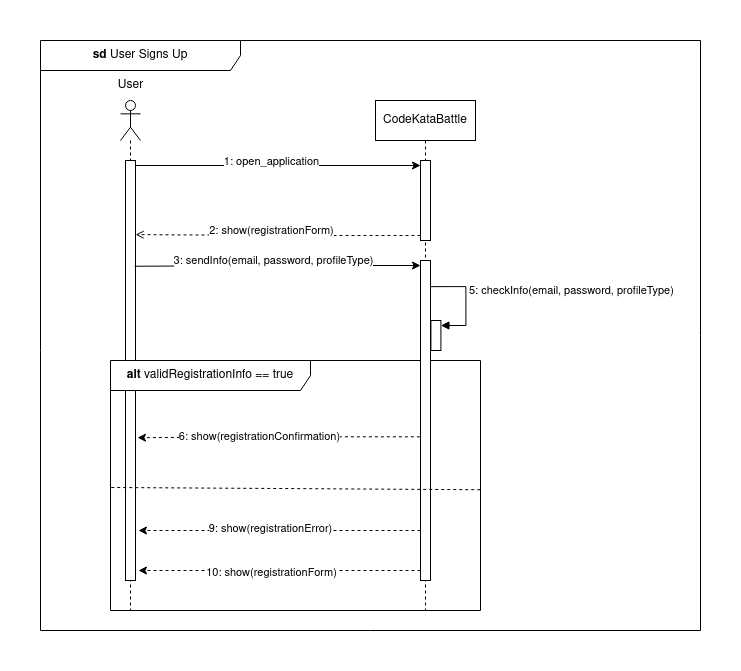
\includegraphics[width=1\linewidth]{misc//Images//UC Diagrams/UC1.png}
    \caption{User Signs Up sequence diagram}
    \label{fig:enter-label}
\end{figure}

\subsubsection{UC2: Log Into Platform}
\begin{center}
    \begin{longtable}{lp{0.75\linewidth}}
        \hline
            Actor & User\\
        \hline
            Entry condition & User is signed into platform\\
        \hline
            Event Flow & 1. User reaches the platform\\
                       & 2. User clicks on "log in" button\\
                       & 3. User fills out email and password used during registration\\
                       & 4. User completes login by clicking "confirm" button\\
        \hline
            Exit & User is successfully logged into platform\\
        \hline
            Exception & Missing or wrong input by user during log in form\\
        \hline
    \end{longtable}
\end{center}

\begin{figure}[H]
    \centering
    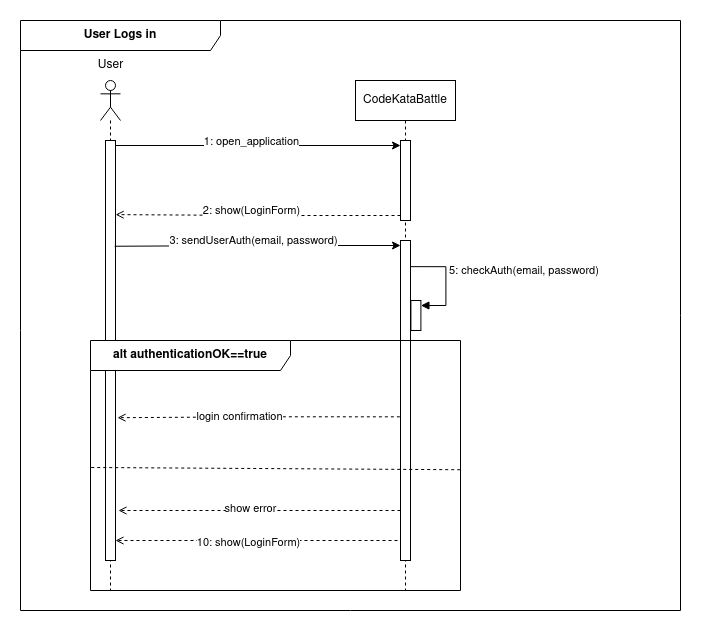
\includegraphics[width=1\linewidth]{misc//Images//UC Diagrams/UC2.png}
    \caption{Create tournament sequence diagram}
    \label{fig:enter-label}
\end{figure}

\newpage
\subsubsection{UC3: Create Tournament}
\begin{center}
    \begin{longtable}{lp{0.75\linewidth}}
        \hline
            Actor & Educator, Students\\
        \hline
            Entry condition & Educator is logged into the platform\\
        \hline
            Event Flow &  1. Educator presses "Create Tournament" button\\
                       &  2. Educator fills out details of tournament\\
                       &  3. Educator adds other collaborators to tournament(other Educators)\\
                       &  4. Educator completes tournament creation\\
                       &  5. Platform notifies all Students of new tournament\\
        \hline
            Exit & Tournament is created successfully \\
        \hline
            Exception & Missing or wrong input by Educator during tournament creation form\\
        \hline
    \end{longtable}
\end{center}

\begin{figure}[H]
    \centering
    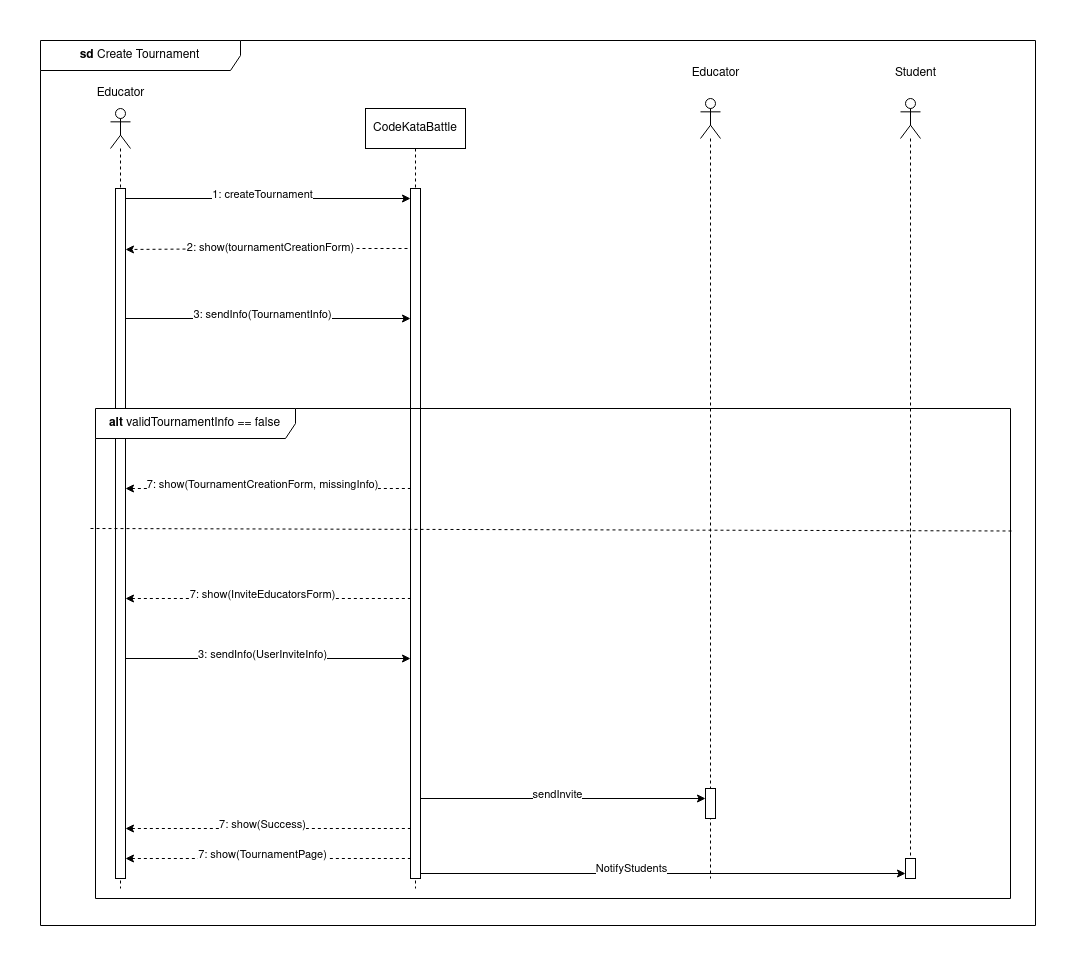
\includegraphics[width=1\linewidth]{misc//Images//UC Diagrams/UC3.png}
    \caption{Create tournament sequence diagram}
    \label{fig:enter-label}
\end{figure}

\newpage
\subsubsection{UC4: Subscribe to Tournament}
\begin{center}
    \begin{longtable}{lp{0.75\linewidth}}
        \hline
            Actor & Students\\
        \hline
            Entry condition & Student is logged into the platform\\
        \hline
            Event Flow & 1. Student is notified of new tournament\\
                       & 2. Student presses "Join tournament" button\\
        \hline
            Exit & Student is subscribed to tournament\\
        \hline
            Exception & \\
        \hline
    \end{longtable}
\end{center}

\begin{figure}[H]
    \centering
    \includegraphics[width=1\linewidth]{misc//Images//UC Diagrams/UC4.png}
    \caption{Subscribe to Tournament sequence diagram}
    \label{fig:enter-label}
\end{figure}

\newpage
\subsubsection{UC5: Create Battle}
\begin{center}
    \begin{longtable}{lp{0.75\linewidth}}
        \hline
            Actor & Educator, Student\\
        \hline
            Entry condition & Educator has logged in and is inside the context of a tournament\\
        \hline
            Event Flow & 1. Educator press "create new battle" button\\
                       & 2. Educator upload the \ac{CK} assignment, tests and project build\\
                       & 3. Educator sets subscription and submission deadlines and group size rules\\
                       & 4. Educator complete battle creation\\
                       & 5. The platform sends notification to all the students subscribed to the tournament\\
        \hline
            Exit & Battle created correctly\\
        \hline
            Exception & Missing or wrong input by Educator\\
        \hline
    \end{longtable}
\end{center}

\begin{figure}[H]
    \centering
    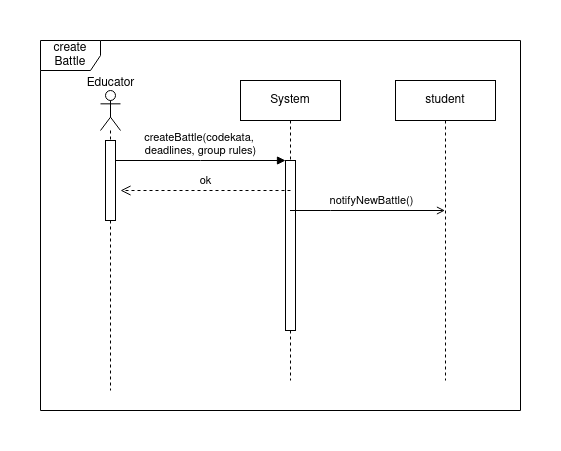
\includegraphics[width=1\linewidth]{misc//Images//UC Diagrams/UC5.png}
    \caption{Create Battle sequence diagram}
    \label{fig:enter-label}
\end{figure}

\newpage
\subsubsection{UC6: Join Battle}
\begin{center}
    \begin{longtable}{lp{0.75\linewidth}}
        \hline
            Actor & Student\\
        \hline
            Entry condition & Student subscribed to a tournament, student logged in, battle available for subscription in tournament\\
        \hline
            Event Flow  & 1. Student press "join battle" button in tournament context\\
                        & 2. platform shows group size rules\\
                        & 3. student uses "invite" button\\
                        & 4. Student inserts other students identifiers\\
                        & 5. other students accepts invite\\
                        & 6. Group of student is created\\
                        & 7. Group of students joins battle\\
        \hline
            Exit & Student group joins battle\\
        \hline
            Exception & \\
        \hline
    \end{longtable}
\end{center}

\begin{figure}[H]
    \centering
    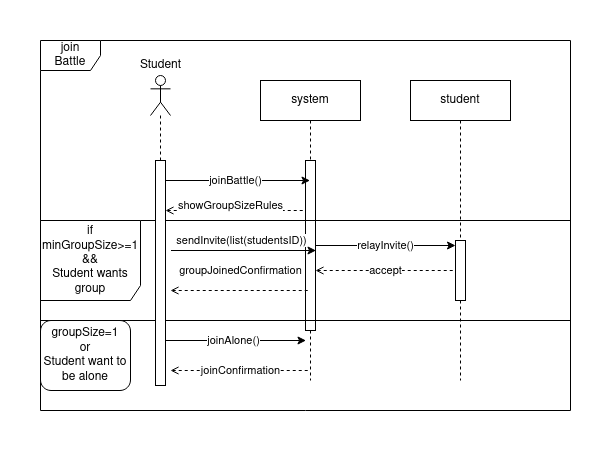
\includegraphics[width=1\linewidth]{misc//Images//UC Diagrams/UC6.png}
    \caption{Join Battle sequence diagram}
    \label{fig:enter-label}
\end{figure}

\newpage
\subsubsection{UC7: Create Repository}
\begin{center}
    \begin{longtable}{lp{0.75\linewidth}}
        \hline
            Actor & Github, Student\\
        \hline
            Entry condition & Subscription deadline of battle expired\\
        \hline
            Event Flow & 1. The platform creates a repository for the codekata battle in github\\
                       & 2. The platform sends to all students subscribed to the battle the link to the repository\\
        \hline
            Exit & Student recieve repository link\\
        \hline
            Exception & \\
        \hline
    \end{longtable}
\end{center}

\begin{figure}[H]
    \centering
    \includegraphics[width=1\linewidth]{misc//Images//UC Diagrams/UC7.png}
    \caption{Create Repository sequence diagram}
    \label{fig:enter-label}
\end{figure}

\newpage
\subsubsection{UC8: Score Commit}
\begin{center}
    \begin{longtable}{lp{0.75\linewidth}}
        \hline
            Actor & GitHub\\
        \hline
            Entry condition & Github notified platform of student commit\\
        \hline
            Event Flow & 1. Platform receives notification of commit\\
                       & 2. Platform pulls sources and compiles them\\
                       & 3. Platform starts evaluation(functional, timeliness, quality)\\
                       & 4. Platform updates score for battle\\
        \hline
            Exit & Battle leader board is updated\\
        \hline
            Exception & Compilation of sources fails\\
        \hline
    \end{longtable}
\end{center}

\begin{figure}[H]
    \centering
    \includegraphics[width=1\linewidth]{misc//Images//UC Diagrams/UC8.png}
    \caption{Score Commit sequence diagram}
    \label{fig:enter-label}
\end{figure}

\newpage
\subsubsection{UC9: View Battle Ranking}
\begin{center}
    \begin{longtable}{lp{0.75\linewidth}}
        \hline
            Actor & User(Educators, Students)\\
        \hline
            Entry condition & Educator is involved with tournament of the battle, student has joined battle\\
        \hline
            Event Flow & 1. User press "view ranking" button in battle context\\
                       & 2.platform shows ranking table\\
        \hline
            Exit & User sees ranking table\\
        \hline
            Exception & \\
        \hline
    \end{longtable}
\end{center}

\begin{figure}[H]
    \centering
    \includegraphics[width=1\linewidth]{misc//Images//UC Diagrams/UC9.png}
    \caption{View Battle Ranking sequence diagram}
    \label{fig:enter-label}
\end{figure}

\newpage
\subsubsection{UC10: Manual Evaluation}
\begin{center}
    \begin{longtable}{lp{0.75\linewidth}}
        \hline
            Actor & Educators\\
        \hline
            Entry condition & Battle deadline Expires\\
        \hline
            Event Flow & 1. Platform notifies educators that battle ha ended and manual evaluation is required(as decided during battle creation)\\
                       & 2. Educators use platform to analyze sources\\
        \hline
            Exit & Educator add a manual score\\
        \hline
            Exception & Educator adds illegal score\\
        \hline
    \end{longtable}
\end{center}

\begin{figure}[H]
    \centering
    \includegraphics[width=1\linewidth]{misc//Images//UC Diagrams/UC10.png}
    \caption{Manual Evaluation sequence diagram}
    \label{fig:enter-label}
\end{figure}

\newpage
\subsubsection{UC11: Look at tournament ranks}
\begin{center}
    \begin{longtable}{lp{0.75\linewidth}}
        \hline
            Actor & Students, Educators\\
        \hline
            Entry condition & Student or Educator are on the main tournament page and are involved\\
        \hline
            Event Flow & 	Student or educator click on tournament leader-board\\
        \hline
            Exit & 	Platform shows Tournament leader board\\
        \hline
            Exception & Tournament hasn't yet started \\
        \hline
    \end{longtable}
\end{center}

\begin{figure}[H]
    \centering
    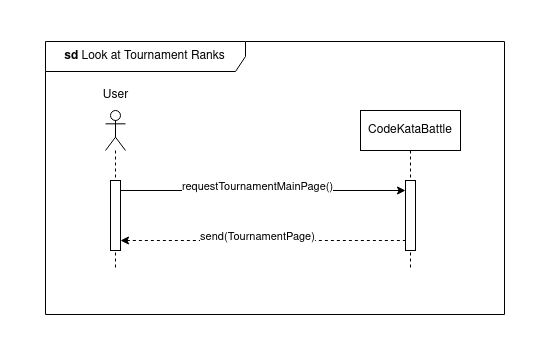
\includegraphics[width=1\linewidth]{misc//Images//UC Diagrams/UC11.png}
    \caption{Look at tournament ranks sequence diagram}
    \label{fig:enter-label}
\end{figure}

\newpage
\subsubsection{UC12: Close Tournament}
\begin{center}
    \begin{longtable}{lp{0.75\linewidth}}
        \hline
            Actor & Educator, Student\\
        \hline
            Entry condition & Educator logged in, Tournament still ongoing, no ongoing battle\\
        \hline
            Event Flow & 1. Edu press "close tournament" in the tournament context\\
& 2. The platform closes the tournament\\
& 3. The platform notifies all the students subscribed to the tournament\\
        \hline
            Exit & Tournament closed, platform notifies students\\
        \hline
            Exception & \\
        \hline
    \end{longtable}
\end{center}

\begin{figure}[H]
    \centering
    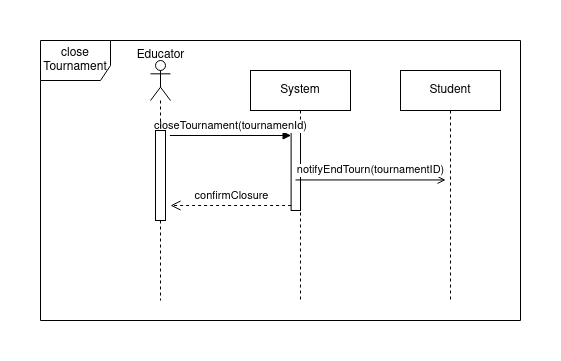
\includegraphics[width=1\linewidth]{misc//Images//UC Diagrams/UC12.png}
    \caption{Close Tournament sequence diagram}
    \label{fig:enter-label}
\end{figure}


\newpage
\subsection{Mapping on requirements}

\begin{center}
    \begin{longtable}{l p{0.75\linewidth}}
        \hline
            \textbf{Use Case} & \textbf{Requirements}\\
        \hline
            UC1 & R10\\
        \hline
            UC2 & R5, R6\\
        \hline
            UC3 & R6, R2.1, R1, R14\\
        \hline
            UC4 & R5, R3\\
        \hline
            UC5 & R6, R2, R2.1, R2.2, R2.3, R2.4, R2.5, R15\\
        \hline
            UC6 & R5, R4, R4.1, R15\\
        \hline
            UC7 & R18, R19\\
        \hline
            UC8 & R9, R9.1, R13, R13.1\\
        \hline
            UC9 & R5, R6, R13, R13.1\\
        \hline
            UC10 & R6, R7, R2.5, R16\\
        \hline
            UC11 & R5, R6, R8, R8.1\\
        \hline
            UC12 & R6, R17, R11\\
        \hline
        
    \end{longtable}
\end{center}

\section{Design Constraints}
\subsection{Standards compliance}
First of all, the system should respect all the laws regarding privacy and data treatment and exchange with third parties (i.e. CPOs); to work in Europe, the system should respect the EU GDPR. In particular, a general description of the main principles that data should have in order to guarantee their privacy is given in Art. 5 of the GDPR document.

\subsection{Hardware limitations}
There are no hardware contraints.

\subsection{Any other constraint}
There are no other constraints.

\section{Software System Attributes}
\subsection{Reliability}
The system should be able to restart automaticly shortly after an interruption and recover the previous backupped state.

\subsection{Availability}
The system should be operative at least 99\% of the time to avoid the impairment of activities with deadlines and in case of downtime the system should recover any missed notification received from GitHub on group commit in battles when it restarts.

\subsection{Security}
The system should ensure safety of the user credentials and it should keep log of access and of sensible operations, such as in the case of educator closing a tournament or manually evaluation of sources, to avoid malicious use of the educator authority.

\subsection{Maintainability}
The development should follow good practice for maintainability, such as dividing the system in enough modules depending on the functionalities. This is necessary in order to facilitate maintenance and substitution of modules. Every functionality needs to be well documented.

\subsection{Portability}
The platform as a website should behave as expected on at least the most used browsers, without requiring additional effort from the end user. The back end should be written in a language that ensures portability and its functionalities should not be reliant on a particular compiler of system.

\newpage

\chapter{Implementation, Integration and Test Plan}
\section{Implementation \& Integration}
The implementation and integration plan will follow a very simple strategy:
\begin{itemize}
    \item First we start by developing the various Microservices of our system: Tournament Service, Battle Service, Leaderboard Service, Invitation Service, Software Evaluation Service, Manual Evaluation Service, Github Handler Service.
    \item Next we make sure the communication with the various DBs works
    \item Then after testing the basic functionalities we will start making our services communicate with the external world by connecting the notification service to an email provider and the GitHub Handler Service to GitHub
    \item Lastly we implement the User side of things, the API gateway and the WebApp
\end{itemize}

\section{Test Plan}
The system should be tested statically during development and dynamically with particular dedication to ensure that no vulnerabilities are left open. For example one of the main security weak point is the Software Evaluation Service as it runs any external code which could eventually be malicious. Regarding the UI/UX side of things it is crucial that the application will be intuitive enough to ensure a good user experience.
\newpage

\chapter{Effort spent}

\begin{table}[h]
    \centering
    \scalebox{1.5}{
    \begin{tabular}{|c | c | c|}
    \hline
        \textbf{Chapter} & \textbf{Valentino} & \textbf{Zarbo} \\ \hline
        1 & 3 & 2\\ \hline
        2 & 16 & 20\\ \hline
        3 & 3 & 5\\ \hline
        4 & 7 & 2 \\ \hline
        5 & 4 & 4\\ \hline
    \end{tabular}
    }
    \caption{Time Spent in hours for each chapter}
    \label{tab:my_label}
\end{table}


\newpage

\chapter{References}
\section{Used tools}
\begin{itemize}
    \item \href{https://github.com/}{GitHub} for project versioning
    \item \href{https://www.overleaf.com}{Overleaf} as \LaTeX\ editor
    \item \href{https://www.jetbrains.com/idea/}{IntelliJ Idea} as Java IDE
\end{itemize}

\end{document}
